\documentstyle[epsf]{book}
\topmargin .5in
\textheight 7.5in
\textwidth 5.5in
\evensidemargin .5in
\oddsidemargin .5in

\makeindex

% Define mathematical symbols and notation
\def\RE{\mathop{\rm I\mkern-3.2mu R}\nolimits}
\def\FE{\mathop{\rm I\mkern-3.2mu F}\nolimits}
\def\CO{\mathop{\rm \mkern0.7mu \raisebox{0.5pt}{\hbox{\vrule height 7pt}}
   \mkern-5.5mu C}\nolimits}
\def\rddots{\mathinner{\mkern1mu\raise1pt\vbox{\kern7pt\hbox{.}}\mkern2mu
   \raise4pt\hbox{.}\mkern2mu\raise7pt\hbox{.}\mkern1mu}}
\def\beq{\begin{eqnarray}}
\def\eeq{\end{eqnarray}}
\def\beqn{\begin{eqnarray*}}
\def\eeqn{\end{eqnarray*}}
\def\beqf{
  \newlength{\lll}
  \setlength{\lll}{\textwidth}
  \addtolength{\lll}{-2\fboxsep}
  \addtolength{\lll}{-2\fboxrule}
  \noindent
  \fbox{%
  \begin{minipage}{\lll}
  \vspace{-\abovedisplayskip}
  }
\def\eeqf{\end{minipage}}}
\def\bfr{\begin{flushright}}
\def\efr{\end{flushright}}
\def\bfl{\begin{flushleft}}
\def\efl{\end{flushleft}}
\def\bq{\begin{quote}}
\def\eq{\end{quote}}
\def\bt{\begin{center}
        \begin{tabular}}
\def\et{\end{tabular}
        \end{center}}
\def\keseq#1{\underline{#1}}

\newcommand{\diag}{{\rm diag}}
\newcommand{\fl}{{\rm fl}}
\newcommand{\In}{{\rm In}}
\newcommand{\Null}{{\cal N}}
\newcommand{\Pf}{\bfl {\it Proof:} \efl}
\newcommand{\Pfend}{\bfr $\diamondsuit$ SDG $\diamondsuit$ \efr}
\newcommand{\Ra}{{\cal R}}
\newcommand{\rank}{{\rm rank}}
\newcommand{\REn}{\RE^n}
\newcommand{\REm}{\RE^m}
\newcommand{\REnn}{\RE^{n \times n}}
\newcommand{\REmm}{\RE^{m \times m}}
\newcommand{\REmn}{\RE^{m \times n}}
\newcommand{\REnm}{\RE^{n \times m}}
\newcommand{\REmnr}{\RE^{m \times n}_r}
\newcommand{\sgn}{{\rm sgn}}
\newcommand{\sig}{{\rm sig}}
\newcommand{\Sp}{{\rm Sp}}
\newcommand{\Tr}{{\rm Tr}}
\newcommand{\vvec}{{\rm vec}}

\newcommand{\no}{\noindent}  
\newcommand{\ba}{\left[ \begin{array}}  
\newcommand{\ea}{\\ \end{array} \right]}  
\newcommand{\bb}{\cite} 
\newcommand{\VE}[1]{\in {\bf R}^{{#1}}} 
\newcommand{\EP}[2]{\in {\bf R}^{{#1} \times {#2}}}
\newcommand{\diago}{\mbox{\rm diag}}
\newcommand{\gammaopt}{\gamma_{opt}}
\newcommand{\xopt}{x_{opt}}
\newcommand{\xgam}{x(\gamma)}
\newtheorem{problem}{Problem}
\newlength{\lll}

\title{
  {\Huge
  Keith On \ldots \\
  \huge
  Numerical Analysis
  \normalsize}
}
\author{
  K.E. Schubert \\
  Visiting Assistant Professor \\
  Department of Mathematics \\
  University of Redlands
}
\date{}

\begin{document}

\newtheorem{definition}{Definition}[chapter]
\newtheorem{theorem}[definition]{Theorem}
\newtheorem{lemma}[definition]{Lemma}
\newtheorem{corollary}[definition]{Corollary}
\baselineskip=1.05\normalbaselineskip

\maketitle
\tableofcontents
\listoffigures
\listoftables
\newpage


\pagenumbering{arabic}

\chapter{Preliminaries}\label{c-Prelim}
%\chapter{Preliminaries}\label{c-Prelim}

\section{Taylor Polynomials}
We want an easier way of calculating a difficult function, $f(x)$.  To this end we want to find a function that is similar to our original that we can calculate.  Taylor polynomials, $p_n(x)$\footnote{The subscript $n$ tells the highest power of the polynomial, i.e. $x^n$.}, are one such type of functions with an easy calculation and intuition.  To find the Taylor polynomials we match the derivatives of the two polynomials at a particular point.  We are in essence enforcing a smoothness criterion at the point of interest, say $x=a$.
\beqn
p_n'(a) &=& f'(a) \\
p_n''(a) &=& f''(a) \\
&\vdots & \\
p_n^{(n)}(a) &=& f^{(n)}(a)
\eeqn
Thus the general expression for the Taylor series is
\beqn
p_n(x) &=& f(a)+(x-a)f'(a)+\frac{(x-a)^2}{2!}f''(a)+\ldots+\frac{(x-a)^n}{n!}f^{(n)}(a) \\
&=& \sum_{k=0}^{n}\frac{(x-a)^k}{k!}f^{(k)}(a)
\eeqn

\textbf{Example}

Problem 1.1-3(c)
\beqn
f(x) &=& \sqrt{1+x} \\
f(0) &=& \sqrt{1+0}=1 \\
f'(0) &=& \frac{1}{2\sqrt{1+0}}=\frac{1}{2} \\
f''(0) &=& \frac{-1}{4(\sqrt{1+0})^3}=\frac{-1}{4} \\
f''(0) &=& \frac{3}{8(\sqrt{1+0})^5}=\frac{3}{8} \\
f^{(k)}(0) &=& \frac{(-1)^{k-1}(2k-3)}{2^k}
\eeqn

\begin{figure}
  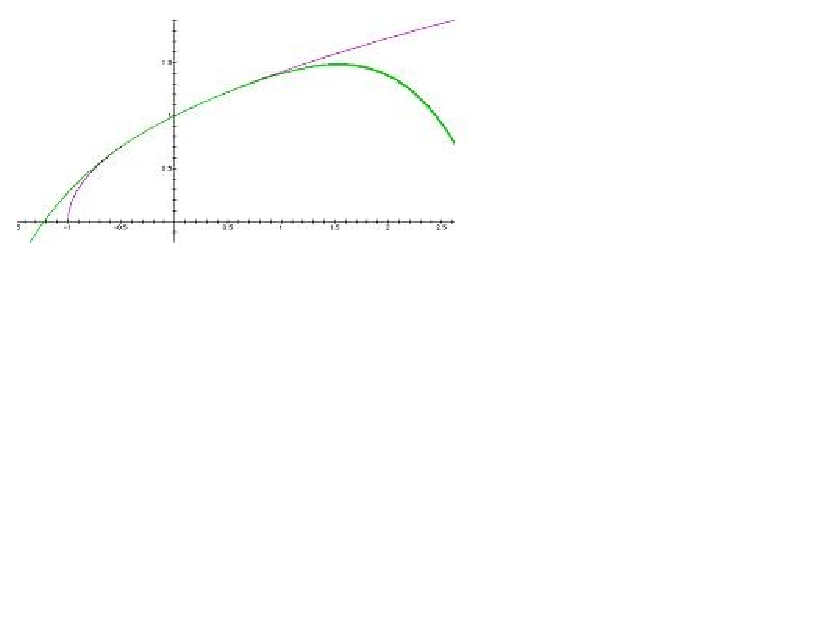
\includegraphics[width=4in]{taylorfit.eps}\\
  \caption{Taylor polynomial and $\sqrt{1+x}$}\label{f-taylor1}
\end{figure}



\textbf{Example}

Problem 1.1-8
\beqn
f(x) &=& \frac{\log(1+x)}{x} \\
&\approx & \frac{\sum_{k=1}^n\frac{(-1)^{k-1}}{k}x^k}{x} \\
&=& \sum_{k=1}^n\frac{(-1)^{k-1}}{k}x^{k-1} \\
f(0) &\approx & 1
\eeqn


\section{Remainder}
The Taylor Series obviously has errors in its approximation.  If the
original function is in $C_{n+1}$ on the interval $\alpha\leq x\leq\beta$ (with $a$ in the
interval) then the remainder (or error) is given by
\beqn
R_n(x) &=& f(x)-p_n(x) \\
&=& \frac{(x-a)^{n+1}}{(n+1)!}f^{(n+1)}(c_x)
\eeqn
with $c_x$ between $a$ and $x$.  To get an error bound we assume that $c_x$ is the worst possible.

\textbf{Example}

Problem 1.2-3(a)
In this case $n=1$ so the worst case would be if $\cos(c_x)=-1$ were $-1$.
\beqn
R_n(x)=\frac{x^{2(1)+1}}{(2(1)+1)!}=\frac{x^3}{6}\leq\frac{\pi^3}{324}<0.081
\eeqn

\textbf{Example}

Prove problem 8.


\section{Evaluating Polynomials}

Consider the polynomial
\beqn
y=a_nx^n+a_{n-1}x^{n-1}+\ldots+a_1x+a_0
\eeqn

\subsection{Straightforward}
The obvious way is to calculate each term separately,
\beqn
a_kx^k=a_k*x*x*...*x
\eeqn
This takes $k$ multiplications for a monomial of size $k$, so for a polynomial with monomials up to size $n$ it would take $\frac{n(n+1)}{2}$ multiplications.

\subsection{Storing}
Calculate $x2=x*x$, $x3=x*x2$, etc. This takes $2n-1$ multiplications.  This is much better that the straightforward way.  We can even do this without having to store each intermediate result by using a temporary variable.  Still it is not the best.

\subsection{Nesting}

Rewrite the polynomial as
\beqn
y&=&a_nx^n+a_{n-1}x^{n-1}+\ldots+a_1x+a_0 \\
&=&((\ldots(((a_n)x+a_{n-1})x+a_{n-2})\ldots)x+a_1)x+a_0.
\eeqn
This can be done as
\beqn
b_n&=&a_n \\
b_{n-1}&=&b_nx+a_{n-1} \\
b_{n-2}&=&b_{n-1}x+a_{n-2} \\
&\vdots & \\
b_1&=&b_2x+a_1 \\
b_0&=&b_1x+a_0
\eeqn
Each step takes 1 multiply so this method takes only n multiplications.  The real savings come when you have to calculate a large polynomial many times.  Another interesting thing is this is a more accurate method,  see Fig~\ref{f-polyeval}, where the dark blue line is the nested multiplication method.  Note on the right side both methods are equally good (or bad in my opinion), but on the right the nested multiplication technique shows marked improvement in accuracy.  Not bad for less work.


\begin{figure}[h]
  % Requires \usepackage{graphicx}
  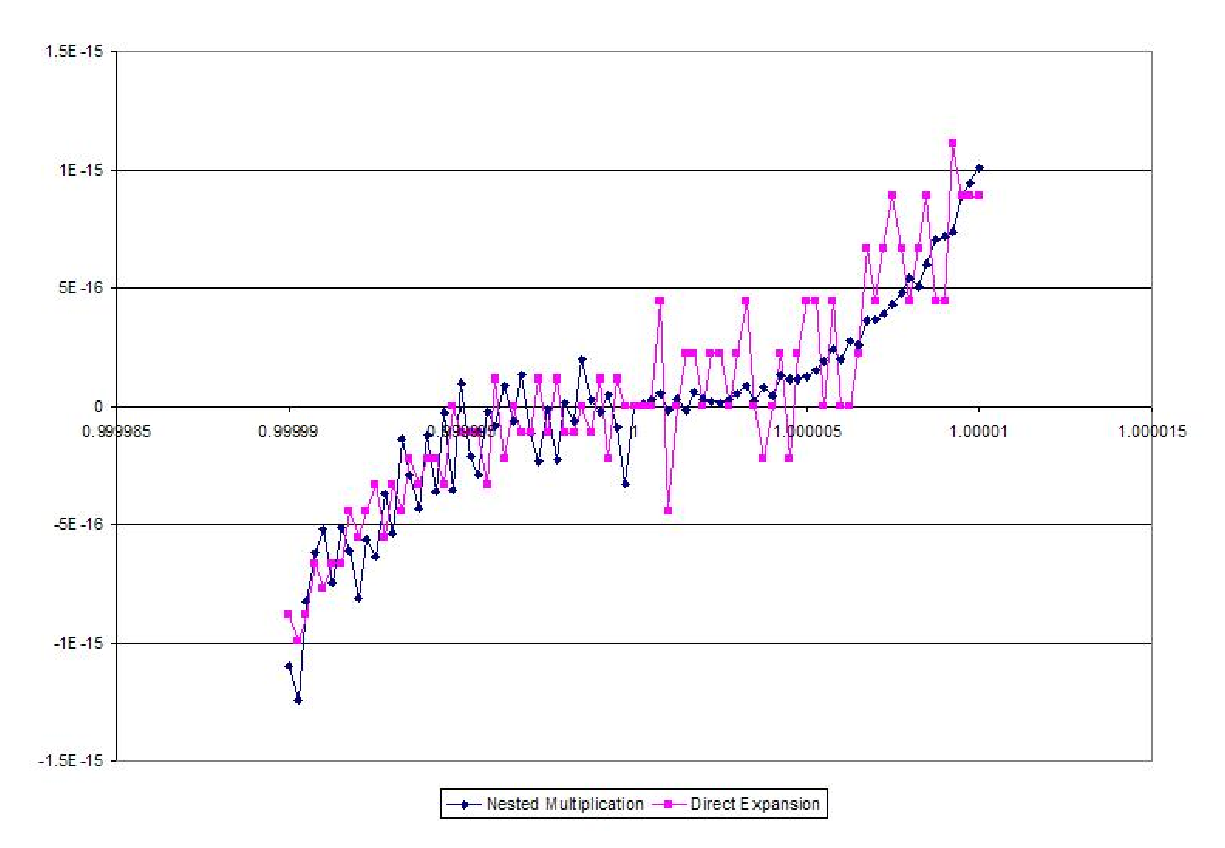
\includegraphics[width=4in]{cubicpoly.eps}\\
  \caption{Close-up Look at Resulting Values of Two Evaluation Methods for $y=x^3-3x^2+3x-1$}\label{f-polyeval}
\end{figure}



\section{Binary}
In any number system, the position of a digit relative to the decimal place specifies the integer power of the base we must multiple the digit by to get its value.  We specify what base we are using by a subscript, if no subscript appears then the base is obvious(usually base 10, though sometimes it will be base 2 if we are calculating in base 2 for that section).  So for base 10
\beqn
101_{10}=1\times 10^2 + 0\times 10^1 + 1\times 10^0,
\eeqn
and for base 2
\beqn
101_2=1\times 2^2 + 0\times 2^1 + 1\times 2^0=5_{10}.
\eeqn
This gives us one way to convert numbers.  For instance, we can convert
binary to decimal by expanding the binary number in this way.  Thus using
the above to convert binary (10.01) to decimal we find,

Note that the ``2'' we are using is the base of binary in decimal form, and this is why we went from binary to decimal.  In binary, its form would be ``10'' and ten would be ``1010''. Therefore, we could go to binary by, expanding this out with ten in binary.  The problem with this method is it is clumsy to use since we do not do squaring, cubing, etc. easily in base 2.  Another problem is that 0.1 is an infinitely repeating decimal in binary so it is a pain to deal with 10-1!  Instead, we convert decimal to binary as follows.
\begin{enumerate}
\item Split your number into a.b
\item For the whole number part, a
  \begin{enumerate}
  \item Divide 2 into a and note the quotient and remainder as q1,r1 (a=2*q1+r1)
  \item As long as the quotient from above is not zero, divide it by 2 and
record the quotient and remainder as qi,ri (with i denoting the current
step).  Repeat.
  \item The binary equivalent of a is rnrn-1...r2r1.  Basically we have done
our nested polynomial evaluation backwards with x=2, and the coefficients
being the remainders.
  \end{enumerate}
\item For the fractional part (b)
  \begin{enumerate}
  \item Multiply 2*b, and record the unit value as a1.  Denote b-a1=b1.
  \item If bi does not equal zero, multiply it by 2, denoting the units digit
by ai+1 and the difference bi-ai+1=bi+1.  Repeat until the difference is
zero (this may never happen so be looking for patterns to get repeating
fractions).
  \item The fractional part, b, is a1a2a3a4...
\end{enumerate}
\item The full answer is thus rnrn-1...r2r1.a1a2a3a4...
\end{enumerate}

\section{Hexadecimal}
This is often made to sound more intimidating than it is.  Hexadecimal
numbers are simply base 16, but this can be handled nicely since $2^4=16$.
All you have to do is group binary digits into groups of 4 and use the
conversion table

\begin{table}
  \centering
  \caption{Binary, Decimal, and Hexadecimal Equivalents}\label{t-bindechex}

\begin{tabular}{|lll|lll|} \hline
Bin  & Hex & Dec & Bin & Hex & Dec \\ \hline
0000 & 0    & 0    & 1000 & 8    & 8    \\
0001 & 1    & 1    & 1001 & 9    & 9    \\
0010 & 2    & 2    & 1010 & A    & 10   \\
0011 & 3    & 3    & 1011 & B    & 11   \\ \hline
0100 & 4    & 4    & 1100 & C    & 12   \\
0101 & 5    & 5    & 1101 & D    & 13   \\
0110 & 6    & 6    & 1110 & E    & 14   \\
0111 & 7    & 7    & 1111 & F    & 15   \\ \hline
\end{tabular}

\end{table}

\section{Fixed Point Numbers}


\vspace{.1in}\noindent
\textbf{Example:}


Convert $\pi$ to binary and hexadecimal.  Assume you have four
bits before the radix point and 8 bits after the radix point.

Sol:

before the decimal we have $3=0011$

after the decimal

\begin{tabular}{l|l}
$0.1415926\ldots$ & \\
\hline
$0.2831852$ & 0 \\
$0.5663704$ & 0 \\
$1.1327408$ & 1 \\
$0.2654816$ & 0 \\
$0.5309632$ & 0 \\
$1.0619264$ & 1 \\
$0.1238528$ & 0 \\
$0.2477056$ & 0 \\
\end{tabular}

combining gives $0011.00100100$

To convert to hexadecimal we group the digits together in groups of four starting at the radix point, thus we are forcing the hexadecimal digits to represent either integer or fractional portions.

\begin{tabular}{|c|c|c|}\hline
0011 & 0010 & 0100 \\ \hline
3    & 2    & 4    \\ \hline
\end{tabular}

Thus the answer is $0x3.24$.




\vspace{.1in}\noindent
\textbf{Example:}


Convert 25.6875 to binary.

    {\color{ans}
    \begin{tabular}{r|lcr|l}
    25 & /2 &.& *2 & .6875 \\ \hline
    12 & 1  & &  1 & .375  \\
     6 & 0  & &  0 & .75   \\
     3 & 0  & &  1 & .5    \\
     1 & 1  & &  1 & 0     \\
     0 & 1  & &    &
     \end{tabular}

     11001.1011
    }



\section{Floating point numbers}
While the book discusses single precision numbers, they are essentially never used, as double precision is so much better and readily available.  We will assume IEEE double precision floating point representation, as it is the standard.  IEEE floating point numbers have the form
\beqn
(-1)^s2^E(b_0.b_{-1}b_{-2}\ldots b_{1-p}),
\eeqn
where
\beqn
s&\in& \{0,1\} \\
s&\in& \{0,1\} \\
b_0&=&1 \,(implicitly) \\
b_{-j}&\in& \{0,1\}\forall j\in\{1,2,\ldots p-1\} \\
\eeqn

\begin{tabular}{lrr}
          & \multicolumn{2}{c}{Precision} \\
          & Single         & Double       \\
P         & 24             & 53           \\
$E_{min}$ & -126           & -1022        \\
$E_{max}$ & 127            & 1023         \\
$Bias$    & 127            & 1023         \\
\end{tabular}

Thus IEEE is represented in memory as a sign bit, exponent bits (8 or 11), and mantissa bits (23 or 52).  The mantissa is composed of all the $b_{-j}$.  A few things to note about IEEE arithmetic.
\begin{enumerate}
\item The exponent stored is $E=e-Bias$
\item $\pm 0$ is encoded by $E_{min}-1$ and $f=0$
\item Denormalized numbers are encoded by $E_{min}-1$ and $f\ne 0$
\item $\pm\infty$ is encoded by $E_{max}+1$ and $f=0$
\item NAN is encoded by $E_{max}+1$ and $f\ne 0$
\end{enumerate}

\subsection{Approximating the Reals}
To approximate the real number x, we define the function fl(x) as, 0 when x=0, and the nearest element in floating point to x otherwise.  Finding nearest elements requires a rounding scheme (rounding or ``chopping''/truncating) and a tie breaker procedure (usually round away from zero).

\subsection{Bounding Errors}
To bound the error in approximating the real number $x$, we need to consider the floating point number, $fl(x)$, used to approximate $x$.  First we note that a real number $x$, is written in binary as
\beqn
x=\sigma\cdot f_r\cdot 2^e,
\eeqn
where $\sigma$ is the sign, $f_r$ has as many digits as needed, and $e$ is any integer.  Note that $e$ will be different for IEEE, which normalizes to $1\leq f_r<2$ with an implicit 1 at the start; than the non-standard forms, which normalize to $0.5\leq f_r<1$ with no assumed leading 1.  We will assume that $e$ is within the permitted bounds for simplicity.  The floating-point representation is
\beqn
fl(x)=\sigma\cdot f\cdot 2^e.
\eeqn
We can now write the difference as
\beqn
x-fl(x)=\sigma\cdot (f_r-f)\cdot 2^e.
\eeqn
For the moment, we will consider the difference $f_r-f$.  Note that we are dealing with normalized numbers with $n$ bits of accuracy and an implicit leading 1 (IEEE arithmetic), while the book deals with numbers normalized between a half and one, with no implicit 1, so for us
\beqn
f_r &=& 1.\beta_{-1}\beta_{-2}\beta_{-3}\ldots\beta_{1-n}\beta_{n}\ldots \\
f_r &=& 1.\bar\beta_{-1}\bar\beta_{-2}\bar\beta_{-3}\ldots\bar\beta_{1-n}.
\eeqn
Note that the digit to the left of the decimal in $f$ is assumed to be 1, the only exception is when $f_r=1.1111...$ which would have $f=10.000...0$\footnote{We are forcing the exponent to be the same, otherwise it would always be true for non-zero numbers}.  Technically it would actually have f=1.000...0 and the exponent would be (e+1) but since we are keeping the exponent e we keep the simplification.  Note that this is equivalent to rounding 9.5 to 10.  Anyway, our real concern is the worst case of the difference, which is in all cases given by
\beqn
f_r-f = \pm 0.000\ldots 01.
\eeqn
Note that the 1 is in the $n^th$ place after the decimal\footnote{Explain}.  We rewrite
this using floating point notation as
.
We now stick this back into the expression for the difference between x
and fl(x) and obtain an upper bound by taking absolute value
.
Similarly to get a lower bound we take the negative of the absolute value,
and find

Now we note that the size of x is
.
For the book's form of the mantissa, we would have
.
The relative error is thus
.



\section{Floating Point Dangers}

I came up with the following program in my doctoral work at UCSB.

\begin{verbatim}
#include <iostream>
#include <iomanip>
#include <cmath>

using namespace std;

int main(){
    double pi, e, result;
    int i;

    e=exp(1);

    pi=atan(1)*4;

    result=pi;

    for(i=1;i<53;i++){
        result=sqrt(result);
    }

    for(i=1;i<53;i++){
        result=result*result;
    }

    cout << setiosflags(ios::showpoint | ios::fixed) << setprecision(16);
    cout << "Pi     = " << pi << endl;
    cout << "Result = " << result << endl;
    cout << "e      = " << e << endl;

    return 0;
}
\end{verbatim}

The results are

\begin{verbatim}
Pi     = 3.1415926535897931
Result = 2.7182818081824731
e      = 2.7182818284590451
Press any key to continue
\end{verbatim}

Notice that Result is $e$ to 7 significant digits, but it should be $\pi$.  This underscores the importance of being numerically aware when writing programs.


\section{IEEE 754}

Floating point numbers are based off scientific notation.  Consider a typical number in base 10 scientific notation,
\begin{eqnarray*}
  -1.23 \times 10^{3}.
\end{eqnarray*}
The number is composed of five pieces of information,
\begin{enumerate}
    \item sign of the number (-),
    \item significant or mantissa (1.23),
    \item base (10),
    \item sign of the exponent (+),
    \item magnitude of the exponent (3).
\end{enumerate}


There are two basic number formats called out in IEEE 754, single precision (float in c/c++), and double precision (double in c/c++).  In addition there are two extended formats, which are only used as intermediate results while calculating.
\vspace{6pt}

\begin{table}
  \centering
  \caption{IEEE Single Precision Floating Point}\label{t-ieee-fp}

\begin{tabular}{|c|c|c|c|}
  \hline
   e & f & Category & Interpretation \\
  \hline
    & $1\ldots 11$ & &  \\
   $1\ldots 11$ & $\vdots$ & NaN & See Codes \\
    & $0\ldots 01$ & &  \\ \hline
   $1\ldots 11$ & $0\ldots 00$ & $\pm\infty$ & $\pm\infty$ \\ \hline
   $1\ldots 10$ & $1\ldots 11$ & &  \\
   $\vdots$ & $\vdots$ & Numbers & $(-1)^s\times 1.f \times 2^{(e-127)}$ \\
   $0\ldots 01$ & $0\ldots 00$ & &  \\ \hline
    & $1\ldots 11$ & &  \\
   $0\ldots 00$ & $\vdots$ & Denormals & $(-1)^s\times 0.f \times 2^{(-126)}$ \\
    & $0\ldots 00$ & &  \\ \hline
   $0\ldots 00$ & $0\ldots 00$ & $\pm 0$ & $\pm 0$ \\ \hline
\end{tabular}
\end{table}


\begin{table}
  \centering
  \caption{IEEE Floating Point NaN Codes}\label{t-ieee-fp-nan}

\begin{tabular}{|c|c|c|}
  \hline
  Dec & Meaning                & Example \\ \hline
  1   & invalid square root    & $\sqrt{-1}$ \\
  2   & invalid addition       & $\infty + -\infty$ \\
  4   & invalid division       & $\frac{0}{0}$ \\
  8   & invalid multiplication & $0\times\infty$ \\
  9   & invalid modulo         & $x mod 0$ \\
   \hline
\end{tabular}
\end{table}

For this discussion, the notation $fl(x)$ will be used to mean the number $x$ as it is represented in floating point on a computer.


$$
(-1)^s\cdot 1.f\times 2^{e-127}
$$

\noindent
\begin{tabular}{c@{\extracolsep{5pt}}c@{}c@{}c@{}c@{}c@{}c@{}c@{}c@{}c@{}c@{}c@{}c@{}c@{}c@{}c@{}c@{}c@{}c@{}c@{}c@{}c@{}c@{}c@{}c@{}c@{}c@{}c@{}c@{}c@{}c@{}c}
  0 & 0 & 0 & 0 & 0 & 0 & 0 & 0 & 0 & 1 & 1 & 1 & 1 & 1 & 1 & 1 & 1 & 1 & 1 & 2 & 2 & 2 & 2 & 2 & 2 & 2 & 2 & 2 & 2 & 3 & 3 & 3 \\
  1 & 2 & 3 & 4 & 5 & 6 & 7 & 8 & 9 & 0 & 1 & 2 & 3 & 4 & 5 & 6 & 7 & 8 & 9 & 0 & 1 & 2 & 3 & 4 & 5 & 6 & 7 & 8 & 9 & 0 & 1 & 2 \\
  \hline
  \multicolumn{1}{|c}{s} & \multicolumn{8}{|c}{e} & \multicolumn{23}{|c|}{f} \\
  \hline
\end{tabular}


This is equivalent to saying


$$
(-1)^s\cdot 1.f\times 2^E
$$

\noindent
\begin{tabular}{c@{\extracolsep{5pt}}c@{}c@{}c@{}c@{}c@{}c@{}c@{}c@{}c@{}c@{}c@{}c@{}c@{}c@{}c@{}c@{}c@{}c@{}c@{}c@{}c@{}c@{}c@{}c@{}c@{}c@{}c@{}c@{}c@{}c@{}c}
  0 & 0 & 0 & 0 & 0 & 0 & 0 & 0 & 0 & 1 & 1 & 1 & 1 & 1 & 1 & 1 & 1 & 1 & 1 & 2 & 2 & 2 & 2 & 2 & 2 & 2 & 2 & 2 & 2 & 3 & 3 & 3 \\
  1 & 2 & 3 & 4 & 5 & 6 & 7 & 8 & 9 & 0 & 1 & 2 & 3 & 4 & 5 & 6 & 7 & 8 & 9 & 0 & 1 & 2 & 3 & 4 & 5 & 6 & 7 & 8 & 9 & 0 & 1 & 2 \\
  \hline
  \multicolumn{1}{|c}{s} & \multicolumn{8}{|c}{e=E+127} & \multicolumn{23}{|c|}{f} \\
  \hline
\end{tabular}

They are the same because $e-127=E$ is the same equation as $e=E+127$.  I think the latter is easier to use because you read $E$ from the number and want $e$.  The first form (standard for most texts) involves you guessing what number produced what you are seeing (rather than calculating it).  It is like trying to solve $y=mx+b$ for $y$ given $x$ but using the form $\frac{(y-b)}{m}=x$ to do it.  It works, just not well.  In any case, consider some examples.

\vspace{.1in}\noindent
\textbf{Example:}

Convert $7.892$ to single precision IEEE.

\noindent
Step 1: Convert 7.892 to binary

$7.892 = 111.1110010001011010000111$

%0.892
%1.784
%1.568
%1.136
%0.272
%0.544
%1.088
%0.176
%0.352
%0.704
%1.408
%0.816
%1.632
%1.264
%0.528
%1.056
%0.112
%0.224
%0.448
%0.896
%1.792
%1.584
%1.168

\noindent
Step 2: Normalize and note sign

$7.892 =(-1)^0 1.111110010001011010000111\times 2^2$

\noindent
Step 3: Calculate Excess 127 code for exponent

$e=2+127=129=10000001$

\noindent
Step 4:Round $1.f$ to 24 digits

$fl(1.111110010001011010000111)=1.11111001000101101000100$

\noindent
Step 5: Assemble


\begin{tabular}{|c@{ }|c@{\extracolsep{5pt}}c@{}c@{}c@{}c@{}c@{}c@{}c@{ \extracolsep{0pt}}|c@{\extracolsep{5pt}}c@{}c@{}c@{}c@{}c@{}c@{}c@{}c@{}c@{}c@{}c@{}c@{}c@{}c@{}c@{}c@{}c@{}c@{}c@{}c@{}c@{}c|}
\hline
0 & 1 & 0 & 0 & 0 & 0 & 0 & 0 & 1 & 1 & 1 & 1 & 1 & 1 & 0 & 0 & 1 & 0 & 0 & 0 & 1 & 0 & 1 & 1 & 0 & 1 & 0 & 0 & 0 & 1 & 0 & 0 \\
  \hline
\end{tabular}



\vspace{.1in}\noindent
\textbf{Example:}


Calculate $3.75\times 29.625$ in IEEE-754 single precision floating point.

    {\color{ans}
    Convert:

    $3.75=11.11=1.111\times 2^1$

    $29.625=11101.101=1.1101101\times 2^4$

    \vspace{12pt}
    Multiply Significants:

    \vspace{6pt}
    \begin{tabular}{cccccccccccc}
     &1.&1&1&0&1&1&0&1& & &  \\
$\times$&1.&1&1&1& & & & & & &  \\ \hline
     &1.&1&1&0&1&1&0&1& & &  \\
     &0.&1&1&1&0&1&1&0&1& &  \\
     &0.&0&1&1&1&0&1&1&0&1&  \\
     &0.&0&0&1&1&1&0&1&1&0&1 \\ \hline
    1&1.&0&1&1&1&1&0&0&0&1&1
    \end{tabular}

    $1.10111100011\times 2^1$

    \vspace{12pt}
    Add exponents to normalization exponent and put in excess 127:

    \vspace{6pt}
    $1+4+1+127=133=10000101$

    \vspace{12pt}
    Write in single precision:

    \vspace{6pt}
    \begin{tabular}{|c|c|c|}\hline 0 & 10000101 & 1011 1100 0110 0000 0000 000 \\ \hline \end{tabular}


    }






\vspace{.1in}\noindent
\textbf{Example:}

Perform the following for IEEE-754, single precision
    \begin{enumerate}
        \item Show the representation of $x=93.3125$

        {\color{ans}

        $x=93.125_{10}=1011101.001_2=1.011101001\times 2^6$

\noindent
\begin{tabular}{|c@{\extracolsep{0pt} }|c@{\extracolsep{5pt}}c@{}c@{}c@{}c@{}c@{}c@{}c@{\extracolsep{0pt} }|c@{\extracolsep{5pt}}c@{}c@{}c@{}c@{}c@{}c@{}c@{}c@{}c@{}c@{}c@{}c@{}c@{}c@{}c@{}c@{}c@{}c@{}c@{}c@{}c@{}c|}
\hline                            %
0 & 1 & 0 & 0 & 0 & 0 & 1 & 0 & 1 & 0 & 1 & 1 & 1 & 0 & 1 & 0 & 0 & 1 & 0 & 0 & 0 & 0 & 0 & 0 & 0 & 0 & 0 & 0 & 0 & 0 & 0 & 0 \\
  \hline
\end{tabular}
        }

        \item calculate $x*y$ for $y$ equal to

\noindent
\begin{tabular}{|c@{\extracolsep{0pt} }|c@{\extracolsep{5pt}}c@{}c@{}c@{}c@{}c@{}c@{}c@{\extracolsep{0pt} }|c@{\extracolsep{5pt}}c@{}c@{}c@{}c@{}c@{}c@{}c@{}c@{}c@{}c@{}c@{}c@{}c@{}c@{}c@{}c@{}c@{}c@{}c@{}c@{}c@{}c|}
\hline                            %
0 & 1 & 0 & 0 & 0 & 0 & 0 & 0 & 0 & 0 & 0 & 0 & 0 & 0 & 0 & 0 & 0 & 0 & 0 & 0 & 0 & 0 & 0 & 0 & 0 & 0 & 0 & 0 & 0 & 1 & 0 & 0 \\
  \hline
\end{tabular}

    {\color{ans}
    exponent: 128+133-127=134

    float: shortcut, note that $y$ only has two 1's in the expansion (hidden and near end) and they are farther apart than the length of the significant portion of $x$.  This will cause the $x$ float to be placed starting at these locations.  The comma below notes where the last bit of precision lies.
\begin{eqnarray*}
z_{fl} & = & 1.01110100100000000000101,1101001
\end{eqnarray*}
Note that the first bit after the comma is a 1 so the number gets rounded up.

        z is

\noindent
\begin{tabular}{|c@{\extracolsep{0pt} }|c@{\extracolsep{5pt}}c@{}c@{}c@{}c@{}c@{}c@{}c@{\extracolsep{0pt} }|c@{\extracolsep{5pt}}c@{}c@{}c@{}c@{}c@{}c@{}c@{}c@{}c@{}c@{}c@{}c@{}c@{}c@{}c@{}c@{}c@{}c@{}c@{}c@{}c@{}c|}
\hline                            %
0 & 1 & 0 & 0 & 0 & 0 & 1 & 1 & 0 & 0 & 1 & 1 & 1 & 0 & 1 & 0 & 0 & 1 & 0 & 0 & 0 & 0 & 0 & 0 & 0 & 0 & 0 & 0 & 0 & 1 & 1 & 0 \\
  \hline
\end{tabular}
    }

    \end{enumerate}



\vspace{.1in}\noindent
\textbf{Example:}

Convert 3.03125 to IEEE single precision

    {\color{ans}
    \begin{tabular}{c|ccc|c}
      3 &   & . &   & 03125 \\ \hline
      1 & 1 &   & 0 & 0625  \\
      0 & 1 &   & 0 & 125  \\
        &   &   & 0 & 25  \\
        &   &   & 0 & 5  \\
        &   &   & 1 & 0  \\
    \end{tabular}

    $3.03125_{10}=11.00001_2=1.100001_2\times 2^1$

    $1+127 = 128$

    \begin{tabular}{|c@{ }|c@{\extracolsep{5pt}}c@{}c@{}c@{}c@{}c@{}c@{}c@{ \extracolsep{0pt}}|c@{\extracolsep{5pt}}c@{}c@{}c@{}c@{}c@{}c@{}c@{}c@{}c@{}c@{}c@{}c@{}c@{}c@{}c@{}c@{}c@{}c@{}c@{}c@{}c@{}c|}
\hline
0 & 1 & 0 & 0 & 0 & 0 & 0 & 0 & 0 & 1 & 0 & 0 & 0 & 0 & 1 & 0 & 0 & 0 & 0 & 0 & 0 & 0 & 0 & 0 & 0 & 0 & 0 & 0 & 0 & 0 & 0 & 0 \\
  \hline
\end{tabular}
    }

Now perform the following on your result and

\begin{tabular}{|c@{ }|c@{\extracolsep{5pt}}c@{}c@{}c@{}c@{}c@{}c@{}c@{ \extracolsep{0pt}}|c@{\extracolsep{5pt}}c@{}c@{}c@{}c@{}c@{}c@{}c@{}c@{}c@{}c@{}c@{}c@{}c@{}c@{}c@{}c@{}c@{}c@{}c@{}c@{}c@{}c|}
\hline
0 & 1 & 0 & 0 & 0 & 0 & 1 & 0 & 0 & 0 & 0 & 0 & 0 & 0 & 0 & 0 & 1 & 0 & 0 & 0 & 0 & 0 & 0 & 0 & 1 & 0 & 0 & 0 & 0 & 0 & 0 & 0 \\
  \hline
\end{tabular}
\begin{enumerate}
    \item Addition

    {\color{ans}
    $x=1.0000000100000001_2\times 2^5$

    $y=1.100001_2\times 2^1=0.0001100001_2\times 2^5$

    \begin{eqnarray*}
    x+y & = & 1.0000000100000001_2\times 2^5+0.0001100001_2\times 2^5 \\
        & = & (1.0000000100000001_2+0.0001100001_2)\times 2^5 \\
        & = & (1.0001100101000001_2)\times 2^5
    \end{eqnarray*}

\begin{tabular}{|c@{ }|c@{\extracolsep{5pt}}c@{}c@{}c@{}c@{}c@{}c@{}c@{ \extracolsep{0pt}}|c@{\extracolsep{5pt}}c@{}c@{}c@{}c@{}c@{}c@{}c@{}c@{}c@{}c@{}c@{}c@{}c@{}c@{}c@{}c@{}c@{}c@{}c@{}c@{}c@{}c|}
\hline
0 & 1 & 0 & 0 & 0 & 0 & 1 & 0 & 0 & 0 & 0 & 0 & 1 & 1 & 0 & 0 & 1 & 0 & 1 & 0 & 0 & 0 & 0 & 0 & 1 & 0 & 0 & 0 & 0 & 0 & 0 & 0 \\
  \hline
\end{tabular}
    }

    \item Multiplication
    {\color{ans}

    exponent is $132+128-127=133$

    significant is $1.0000000100000001\times 1.100001 = 1.1000010110000101100001$

\begin{tabular}{|c@{ }|c@{\extracolsep{5pt}}c@{}c@{}c@{}c@{}c@{}c@{}c@{ \extracolsep{0pt}}|c@{\extracolsep{5pt}}c@{}c@{}c@{}c@{}c@{}c@{}c@{}c@{}c@{}c@{}c@{}c@{}c@{}c@{}c@{}c@{}c@{}c@{}c@{}c@{}c@{}c|}
\hline
0 & 1 & 0 & 0 & 0 & 0 & 1 & 0 & 1 & 1 & 0 & 0 & 0 & 0 & 1 & 0 & 1 & 1 & 0 & 0 & 0 & 0 & 1 & 0 & 1 & 1 & 0 & 0 & 0 & 0 & 1 & 0 \\
  \hline
\end{tabular}
    }

\end{enumerate}






\vspace{.1in}\noindent
\textbf{Example:}

Perform the following for IEEE-754, single precision
    \begin{enumerate}
        \item Show the representation of $x=0.8125$

        {\color{ans}

\noindent
\begin{tabular}{|c@{\extracolsep{0pt} }|c@{\extracolsep{5pt}}c@{}c@{}c@{}c@{}c@{}c@{}c@{\extracolsep{0pt} }|c@{\extracolsep{5pt}}c@{}c@{}c@{}c@{}c@{}c@{}c@{}c@{}c@{}c@{}c@{}c@{}c@{}c@{}c@{}c@{}c@{}c@{}c@{}c@{}c@{}c|}
\hline                            %
0 & 0 & 1 & 1 & 1 & 1 & 1 & 1 & 0 & 1 & 0 & 1 & 0 & 0 & 0 & 0 & 0 & 0 & 0 & 0 & 0 & 0 & 0 & 0 & 0 & 0 & 0 & 0 & 0 & 0 & 0 & 0 \\
  \hline
\end{tabular}
        }

        \item calculate (show steps) $x*y$ for $x$ from above and

        y is

\noindent
\begin{tabular}{|c@{\extracolsep{0pt} }|c@{\extracolsep{5pt}}c@{}c@{}c@{}c@{}c@{}c@{}c@{\extracolsep{0pt} }|c@{\extracolsep{5pt}}c@{}c@{}c@{}c@{}c@{}c@{}c@{}c@{}c@{}c@{}c@{}c@{}c@{}c@{}c@{}c@{}c@{}c@{}c@{}c@{}c@{}c|}
\hline                            %
1 & 1 & 0 & 0 & 0 & 0 & 0 & 0 & 1 & 1 & 1 & 0 & 0 & 0 & 0 & 0 & 0 & 0 & 0 & 0 & 0 & 0 & 0 & 0 & 0 & 0 & 0 & 0 & 0 & 0 & 0 & 0 \\
  \hline
\end{tabular}

        {\color{ans}
        Exponent: $(10000001+01111110)-01111111=11111111-01111111=1000000$

        float= $1.101*1.11=10.11011=1.011011 \times 2^1$, so add 1 to exponent

\noindent
\begin{tabular}{|c@{\extracolsep{0pt} }|c@{\extracolsep{5pt}}c@{}c@{}c@{}c@{}c@{}c@{}c@{\extracolsep{0pt} }|c@{\extracolsep{5pt}}c@{}c@{}c@{}c@{}c@{}c@{}c@{}c@{}c@{}c@{}c@{}c@{}c@{}c@{}c@{}c@{}c@{}c@{}c@{}c@{}c@{}c|}
\hline                            %
1 & 1 & 0 & 0 & 0 & 0 & 0 & 0 & 1 & 0 & 1 & 1 & 0 & 1 & 1 & 0 & 0 & 0 & 0 & 0 & 0 & 0 & 0 & 0 & 0 & 0 & 0 & 0 & 0 & 0 & 0 & 0 \\
  \hline
\end{tabular}
        }

        \item Perform the multiplication above in decimal and verify the answer.

        {\color{ans}
        $.8125*(-7)=-5.6875=-101.1011_2$
        }

    \end{enumerate}

\section{Rounding versus Chopping}

Rounding is almost always used because of two reasons.  To see both, let the interval between two numbers in the representation is $2\delta$ then for rounding $x-fl(x)\in [-\delta,\delta)$, while for chopping it is $x-fl(x)\in [0,2\delta)$.  The first problem is that the error magnitude is up to twice as large for chopping.  This is obviously bad, but it is not as bad as the second problem.  The second problem is that all the errors of chopping have the same sign, so no error cancellation is possible when calculations are done.  To see why this is bad, consider the following.

\vspace{.1in}\noindent
\textbf{Example:}

Find out the error in calculating $\sum_{i=1}^{n}x_i$ on a computer.  First note that what you actually calculate is $\sum_{i=1}^{n}fl(x_i)$.  The error (actual minus calculated) is thus $Err=\left|(\sum_{i=1}^{n}x_i)-(\sum_{i=1}^{n}fl(x_i))\right|$.  Also let $fl(x_i)=x_i+\gamma_i$ for $\gamma_i$ in the error interval of your method.

\begin{eqnarray*}
  Err &=& \left|(\sum_{i=1}^{n}x_i)-(\sum_{i=1}^{n}(x_i+\gamma_i))\right| \\
    &=& \left|(\sum_{i=1}^{n}x_i)-(\sum_{i=1}^{n}x_i+\sum_{i=1}^{n}\gamma_i)\right| \\
    &=& \left|\sum_{i=1}^{n}x_i-\sum_{i=1}^{n}x_i-\sum_{i=1}^{n}\gamma_i\right| \\
    &=& \left|\sum_{i=1}^{n}\gamma_i\right| \\
    &\leq & \sum_{i=1}^{n}\left|\gamma_i\right|
\end{eqnarray*}

For chopping the last inequality is actually an equality, i.e. chopping always has the worst case error.  For a typical case on rounding the errors are distributed with some positive and some negative, thus cancelation can occur.  For large sums (many terms) the law of large numbers and an assumed uniform distribution of $\gamma_i$ indicates that the error for rounding will go to $0$!  This is a great result.

\section{Absolute and Relative Error}

The two most basic types of errors are absolute and relative.  The absolute error of an estimate $\hat x$ of a number $x$, is the difference between them.
\begin{eqnarray}
AE&=&\Delta x\\
  &=&x-\hat x
\end{eqnarray}
The relative error of an estimate $\hat x$ of a number $x$, is the difference between them divided by $x$.
\begin{eqnarray}
RE&=&\frac{\Delta x}{x}\\
  &=&\frac{x-\hat x}{x}
\end{eqnarray}
Often the the absolute value of either the absolute or relative error is taken, though not in every case, so it is important to know if only the magnitude or magnitude and phase (sign) is required.  Unfortunately, there is no standard nomenclature or convention, though more often than not the magnitude (take the absolute value) is desired. Usually the phase/sign information is only retained in the error if it is plausible to have and will be useful in the algorithm or analysis.

\section{Propagation of Error}
We have seen that representing the real numbers on a computer involves errors.  When we use floating point numbers in a calculation rather than the actual numbers the errors can grow.  The errors caused by using floating point approximations are called propagated errors.  Two ways of bounding propagation errors exist.  The forward method involves explicitly calculating the errors and is called interval arithmetic.  The backward method involves finding a condition number, which gives a bound on how big the error can grow.

\section{Interval Arithmetic}

Let's consider the error in a computation between the true values (xT, yT) and the approximate values (xA, yA).  We only know the approximate values and the error bounds

Note that the error is could be positive or negative so we must consider the positive and negative bounds.  First, we will look at the error for addition or subtraction.

Now let's consider multiplication.

It is easy to see that this can quickly become very hard to deal with.  Consider for instance multiplying two n-by-n matrices, which would involve $n^{3}$ multiplies.  Keeping track of all of them would rapidly become impossible.  We will consider one final operation, namely division.

Again we can see that things can become very complicated quickly.

\section{Forward and Backward Error}

Two other distinctions in error types that come up in stability of algorithms are forward and backward errors.  They are concerned with a piece of data, $x$, that is acted on by an equation or algorithm, $f(\cdot)$ to produce a result, $y$.
\begin{eqnarray}
y&=&f(x)
\end{eqnarray}
This probably seems pretty straight-forward, but what happens when I can't actually calculate $f(\cdot)$?  For instance, how can I calculate a transcendental function\footnote{Transcendental functions cannot be expressed as a finite sequence of algebraic operations - arithmetic and roots} like $\sin(x)$?  The answer is we have to approximate the equation or algorithm with another one that is calculable on a computer.  We will examine some ways to do this later, but first we need a way to see how good our approximation is, which is what forward and backward errors gives us.  We will denote our approximate algorithm by $\hat f(\cdot)$.  Now if we give our approximate algorithm the true starting value of $x$, what it calculates will not be $y$ but $\hat y$.
\begin{eqnarray}
\hat y&=&\hat f(x)
\end{eqnarray}
The error of the results, given the same starting point, gives us an idea of how good our approximation is.  If it is small then we say the algorithm is stable.  The difference of the values calculated is the forward error.
\begin{eqnarray*}
FE_{abs}&=&\Delta y\\
        &=& y-\hat y\\
        &=& f(x)-\hat(x)\\
FE_{rel}&=&\frac{\Delta y}{y}\\
        &=& \frac{y-\hat y}{y}\\
        &=& \frac{f(x)-\hat f(x)}{f(x)}
\end{eqnarray*}
In general we will use the relative forward error, though you could use either.  Forward error is a useful and intuitive concept, but it is not always easy to quantify for a range of values, since you have to explicitly calculate for each one.  This makes it less useful for algorithm analysis.  Enter the backward error.  Its definition will seem weird and probably even more difficult, but it turns out to be easy in many cases to bound for a wide range of problems.  In other words we use it because it makes our lives easy.

The backward error is the smallest value, $\Delta x$ such that
\begin{eqnarray}
f(\hat x) &=& \hat f(x)\\
\hat x &=& x+\Delta x
\end{eqnarray}
holds.  Solving this we find
\begin{eqnarray*}
f(x+\Delta x) &=& \hat f(x)\\
x+\Delta x &=& f^{-1}\left(\hat f(x)\right)\\
\Delta x &=& f^{-1}\left(\hat f(x)\right)-x.
\end{eqnarray*}
The absolute backward error is $\Delta x$ and the relative backward error is $\frac{\Delta x}{x}$.

\section{Condition Number}
To make this a little more understandable, I am going to draw a distinction not used in the literature\footnote{This warning exists only to prevent you from expecting others to know or use this, though it is much clearer in my mind.}, that of condition number at a point and condition number of an algorithm.  The condition number of an algorithm is the worst condition number at a point for all the possible points, thus
\begin{eqnarray}
cond(f) &=& \sup_x cond(f(x))
\end{eqnarray}
The condition number at a point is then how much the output changes given a change in the input, thus it is a ratio of the relative forward error over the relative backward error.
\begin{eqnarray*}
cond(f(x)) &=& \left|\frac{\frac{y-\hat y}{y}}{\frac{x-\hat x}{x}}\right| \\
           &=& \left|\frac{\frac{f(x)-\hat f(x)}{f(x)}}{\frac{x-f^{-1}(\hat f(x))}{x}}\right|
\end{eqnarray*}
Note that by definition of the backward error, we have $f(\hat x) = \hat f(x)$ and $\Delta x= x-\hat x$.
\begin{eqnarray*}
cond(f(x)) &=& \left|\frac{\frac{f(x)-f(\hat x)}{f(x)}}{\frac{\Delta x}{x}}\right|
\end{eqnarray*}
In this form it looks a lot like a calculus formula, which suggests using the derivative to simplify the equation.  This of course requires the derivative to exist.  Recall that 
\begin{eqnarray*}
f'(x)&=&lim_{\Delta x\rightarrow 0}\frac{f(x)-f(x+\Delta x)}{\Delta x}.
\end{eqnarray*}
We don't have a limit, so we can only approximate this
\begin{eqnarray*}
f'(x)&\approx&\frac{f(x)-f(x+\Delta x)}{\Delta x}
\end{eqnarray*}
thus
\begin{eqnarray*}
cond(f(x)) &=& \left|\frac{\frac{f(x)-f(\hat x)}{f(x)}}{\frac{\Delta x}{x}}\right| \\
           &=& \left|\frac{f(x)-f(\hat x)}{\Delta x}\frac{x}{f(x)}\right| \\
           &=& \left|\frac{f(x)-f(x+\Delta x)}{\Delta x}\frac{x}{f(x)}\right| \\
           &\approx& \left|f'(x)\frac{x}{f(x)}\right|
\end{eqnarray*}
The condition number at a point thus gives us how the errors grow at that point, and the condition number of the function gives us the worst case bound on how bad our errors can grow.

Note this is not the only way we could have developed this.  We could have required our
function to be continuous on [$x$,$\hat x$] and differentiable on ($x$,$\hat x$), which is looser than the completely differentiable requirement I made above.  We can thus use the mean value theorem to see
\begin{eqnarray*}
f'(c)&=&\frac{f(x)-f(\hat x)}{x-\hat x}
\end{eqnarray*}
We now note that since $c$ is between the true, $x$, and approximate, $\hat x$ values, and that the interval is on the order of $10^{-16}$ for IEEE double-precision arithmetic.  We can thus assume $c$ is approximately $x$.
\begin{eqnarray*}
f'(x)&\approx&\frac{f(x)-f(\hat x)}{x-\hat x}
\end{eqnarray*}
The derivative of $f(x)$ at $x$, is called the absolute condition number.  To get the relative condition number you just have to divide each of the differences by their true value, which works out to multiplying by $\frac{x}{f(x)}$, thus
\begin{eqnarray*}
cond(f(x)) &\approx& \left|f'(x)\frac{x}{f(x)}\right|
\end{eqnarray*}
Same equation either way.

The condition number shows how the error of the approximation will influence the error of the calculation.    The condition number is nice in that it cleanly handles the error bounds.  It is not as precise as the error in the interval arithmetic, but it is tractable even for large matrix operations, which will involve the norms of the matrices rather than the elements.  Quite a
savings!

\subsection{Sums}
We have spoken a lot about summation, but we want to look at one final
area of sums before we move on.  Consider the following summation:
\begin{eqnarray}
100000+45+45+45+45
\end{eqnarray}
In real numbers it doesn't matter if we add the 45's first or the 100000.
In floating point numbers it does matter!  Floating point numbers are not
associative.  To see this consider a 4 decimal place accuracy machine that
uses rounding, and is nicely implemented.  In this case we see that
\beqn
100000+45=100000
\eeqn
so if we add as stated we find the sum is 100000 for the series (rather
than 100180).  If we add the 45's first we find that
\beqn
45+45+45+45=180,
\eeqn
then
\beqn
100000+180=100200.
\eeqn
A much better result.  These sums occur in a variety of places, from
standard series, to evaluating integrals, to inner products of vector, and
matrix multiplication.  In short you should be aware of the lack of the
associative property.


\vspace{.1in}\noindent
\textbf{Example}

Write C/C++ code to sum the following $\sum_{i=1}^{100}\frac{1}{i^2}$.  Make sure you do it in the right order.
    {\color{ans}

    \begin{verbatim}
    double sum=0;
    int i;

    for(i=100;i>=0;i--){
        sum+=1.0/(i*i);}
    \end{verbatim}

    }

\subsubsection{Kahan's Compensated Summation}

\SciLab{Kahan's Compensated Summation}{sci:kahan-comp-sum}{scilab/compsum.sci} 
\newpage
\chapter{Zero Finding}\label{c-zero}
Almost every interesting problem in mathematics can be reduced to trying 
to find the zeros of a function.  The next several classes will be spent 
examining how we find zeros.  In general, you cannot explicitly solve for 
the zeros so you need to make iterative procedures to find them.  Today we 
will look at two methods: bisection and Newton's method.
\section{Bisection}
Bisection is a nice method in that it is guaranteed to converge and you 
can state exactly how many iterations it will take.


\section{Newton's Method}
Newton's Method essentially is an algebraic re-writing of the tangent line 
of a function at a point.

We can then use Taylor's formula to obtain an error bound.
\section{Secant}
Newton's Method requires the knowledge of the first derivative of the 
function.  Often the derivative is very complicated to evaluate and 
will take a long (relatively anyway) time to do so.  In many cases the 
first derivative may not be available.  In some cases it might not even 
exist at all points in the interval of interest.  Even when it is 
available it could be near zero which would cause numerical problems 
in evaluating it, even if it is in the region of convergence.  For 
all of these regions a new method was devised, which drew on the 
material leading up to calculus.  

Recall that the tangent line was 
found as the limit of a series of secant lines.  We can say that the 
derivative can thus be approximated by
\beqn
f(x)\approx\frac{f(x_{1})-f(x_{2})}{x_{1}-x_{2}}.
\eeqn
Thus if we know two points, we can approximate the funciton by a 
straight line between them and use the x-intercept as the next point 
to evaluate.  We now need two points instead of one and a 
derivative.  We refer to this as a two-point method because of the 
need of multiple points.  We will need two estimates to begin our 
evaluation.  Given two initial gueses, $x_{0}$ and $x_{1}$, the slope, 
$m$, is given by
\beqn
m=\frac{f(x_{1})-f(x_{0})}{x_{1}-x_{0}}.
\eeqn
Using this we find the next point, $x_{2}$ by using the point-slope 
form of a line
\beqn
f(x_{2})-f(x_{1}) & = & 
  \frac{f(x_{1})-f(x_{0})}{x_{1}-x_{0}}(x_{2}- x_{1}) \\
x_{2}- x_{1} & = & 
  \frac{x_{1}-x_{0}}{f(x_{1})-f(x_{0})}(f(x_{2})-f(x_{1})) \\
x_{2} & = & 
  x_{1}-f(x_{1})\frac{x_{1}-x_{0}}{f(x_{1})-f(x_{0})}. 
\eeqn
We thus have the equation for the next estimate:
\beq
x_{n+1} = 
  x_{n}-f(x_{n})\frac{x_{n}-x_{n-1}}{f(x_{n})-f(x_{n-1})}. \label{eq-sec1}
\eeq
Note that you can store the previous function evaluation and then you 
will not need to do two function evaluations per iteration.

Now we want to calculate the error.  To do this we will subtract 
eq~\ref{eq-sec1} from $\alpha=\alpha$.
\beqn
e_{n+1} & = & \alpha - x_{n+1} \\
  & = & \alpha -
    \left(x_{n}-f(x_{n})\frac{x_{n}-x_{n-1}}{f(x_{n})-f(x_{n-1})}\right) \\
  & = & \alpha -\frac{f(x_{n})x_{n-1}-f(x_{n-1})x_{n}}{f(x_{n})-f(x_{n-1})} \\
  & = & \frac{f(x_{n})(\alpha -x_{n-1})-f(x_{n-1})(\alpha -x_{n})}
       {f(x_{n})-f(x_{n-1})} \\
  & = & \frac{f(x_{n})e_{n-1}-f(x_{n-1})e_{n}}{f(x_{n})-f(x_{n-1})} \\
  & = & e_{n} e_{n-1}\frac{\frac{f(x_{n})}{e_{n}}-\frac{f(x_{n-1})}{e_{n-1}}}
       {f(x_{n})-f(x_{n-1})} \\
  & = & e_{n} e_{n-1}\frac{\frac{f(x_{n})}{e_{n}}-\frac{f(x_{n-1})}{e_{n-1}}}
       {x_{n}-x_{n-1}}\frac{x_{n}-x_{n-1}}{f(x_{n})-f(x_{n-1})} \\
  & \approx & e_{n} e_{n-1}\frac{\frac{f(x_{n})}{e_{n}}-\frac{f(x_{n-1})}{e_{n-1}}}
       {x_{n}-x_{n-1}}\frac{1}{f'(\alpha)}
\eeqn
We need to evaluate $\frac{f(x_{n})}{e_{n}}$, so we will use Taylor's 
Theorem for $f(x)$ evaluated at $\alpha$.  We find that
\beqn
\frac{f(x_{n})}{e_{n}} & = & 
\frac{f(\alpha)+(\alpha-x_{n})f'(\alpha)+\frac{1}{2}
  (\alpha-x_{n})^{2}f''(\alpha)+{\cal O}((\alpha-x_{n})^{3})}{e_{n}} \\
& = & 
\frac{e_{n}f'(\alpha)+\frac{1}{2}e_{n}^{2}f''(\alpha)
   +{\cal O}(e_{n}^{3})}{e_{n}} \\
& = & 
f'(\alpha)+\frac{1}{2}e_{n}f''(\alpha)+{\cal O}(e_{n}^{2})
\eeqn
Resuming our evaluation of $e_{n+1}$ we find
\beqn
e_{n+1} 
  & \approx & e_{n} e_{n-1}\frac
  {f'(\alpha)+\frac{1}{2}e_{n}f''(\alpha)+{\cal O}(e_{n}^{2})
  -f'(\alpha)-\frac{1}{2}e_{n-1}f''(\alpha)+{\cal O}(e_{n-1}^{2})}
       {x_{n}-x_{n-1}}\frac{1}{f'(\alpha)} \\
  & = & e_{n} e_{n-1}\frac{\frac{1}{2}e_{n}f''(\alpha)
   -\frac{1}{2}e_{n-1}f''(\alpha)+{\cal O}(e_{n-1}^{2})}
       {x_{n}-x_{n-1}}\frac{1}{f'(\alpha)} \\
  & = & e_{n} e_{n-1}\frac{\frac{1}{2}(e_{n}-e_{n-1})f''(\alpha)
   +{\cal O}(e_{n-1}^{2})}{x_{n}-x_{n-1}}\frac{1}{f'(\alpha)} \\
  & = & e_{n} e_{n-1}\frac{\frac{1}{2}(x_{n}-x_{n-1})f''(\alpha)
   +{\cal O}(e_{n-1}^{2})}{x_{n}-x_{n-1}}\frac{1}{f'(\alpha)} \\
  & = & e_{n} e_{n-1}(\frac{1}{2}f''(\alpha)
   +{\cal O}(e_{n-1}^{2}))\frac{1}{f'(\alpha)} \\
  & \approx & e_{n}e_{n-1}\frac{f''(\alpha)}{2f'(\alpha)} \\
  & \approx & e_{n}e_{n-1}M.
\eeqn
This is similar to Newton's method which suggests that
\beqn
  e_{n+1}=Ae_{n}^{c},
\eeqn
which implies
\beqn
  e_{n}=A^{-1}e_{n-1}^{c^{-1}}.
\eeqn
Substituting and collecting terms we find
\beqn
B=e_{n}^{1-c+c^{-1}}.
\eeqn
Since the left hand side is a constant the exponent must be zero, or 
$c$ must be the golden ratio.
This implies that the secant method converges superlinearly.
\section{Regula Falsi}


\section{Fixed Points}
A fixed point is a point in the domain of a function, which maps its 
domain back into its domain, that satisfies $\alpha=C(\alpha)$.  
Since $\alpha$ does not change when it is mapped by the function it is 
fixed, hence the name.  We need to look at what 
the idea that underlies fixed points: contractions.  A contraction 
$y=C(x)$, is a mapping from a closed interval in $X$ into another closed 
interval in $Y$ with the property that for some $b=C(a)$ (usually $a$ 
and $b$ are both the origin but it is not required), $\|\cdot\|_{x}$ 
a norm on $X$, and $\|\cdot\|_{y}$ a norm on $Y$ we have:
\beqn
\| x-a\|_{x} > \| y-b\|_{y} = \| C(x)-C(a)\|_{y}
\eeqn
for all $x\in X$ and $y\in Y$.  Usually we have $X$ and $Y$ are $\Re$ 
and $a=b$, which gives us that $|x-a|>|C(x)-a|$.  Take the derivative of both 
sides and we see 
\beqn
1>|C'(x)|.
\eeqn
This brings up a key point, we must have that the magnitude of the 
function's slope is less than 1.  If you think about this it makes 
sense, as for slope magnitudes greater than one there will be growth 
and we are looking a funcions which shrink things.  While this is a 
simple idea, it has many profound implications.  The book proves 
nicely how the uniqueness of solution, convergence, etc..  One thing 
that should be highlated has to do with rate of convergence.  Given a 
contraction defined on an interval $[a,b]$ with some point, $\alpha = 
C(\alpha)\in[a,b]$ called a fixed point, we can define the iteration 
$x_{n+1}=C(x_{n})$.  We then have (using the mean value theorem)
\beqn
\alpha-x_{n+1} 
 & = & C(\alpha)-C(x_{n}) \\
 & = & C'(d)(\alpha-x_{n}) \\
|\alpha-x_{n+1}| 
 & < & |\alpha-x_{n}|.
\eeqn
We have linear convergence from this.  Consider the following paradox.

Let a function $g(x)$ be defined by
\beqn
g(x)=x-\frac{f(x)}{f'(x)}
\eeqn
and let $f(x)$ have a single root in some interval $[a,b]$.  From the 
book we know this must have a fixed point in the interval and the 
iteration $x_{n+1}=g(x_{n})$ will converge to the fixed point.  This 
method thus has linear convergence from what we have proven above.  
This iteration is Newton's Method though, so it has Quadratic 
convergence.  What gives?  The convergence of a fixed point algorithm 
is at least linear but it can be better if $C'(\alpha)=0$.  Notice 
that the derivative of $g(x)$ is given by
\beqn
g'(x) & = & 1-\frac{(f'(x))^{2}-f(x)f''(x)}{(f'(x))^{2}} \\
      & = & \frac{f(x)f''(x)}{(f'(x))^{2}}.
\eeqn
Note that for $x=\alpha$ we trivially have that $g'(\alpha)=0$, which 
satisfies our requirement for faster convergence.

How can I get a function $g(x)$ that satisfies the requirements?  
Many ways exist but consider the following.  For a function $f(x)$ with 
a zero at $x=\alpha$ in an interval $[a,b]$, that has 
$\beta=\max_{x\in[a,b]}|f'(x)|$, we define the iteration
\beqn
x_{n+1}=x_{n}-\gamma sign(f'(x_{n}))f(x_{n})
\eeqn
with $0<\gamma\beta<2$.  We then see that
\beqn
g(x) & = & x-\gamma sign(f'(x))f(x) \\
g'(x) & = & 1-\gamma sign(f'(x))f'(x) \\
      & = & 1-\gamma |f'(x)|
\eeqn
and thus $1>g'(x)>-1$.  Note that if we choose $\gamma$ such that 
$0<\gamma\beta<1$ then $1>g'(x)>0$ and the sequence 
$\{x_{i}\}_{i=0}^{\infty}$ converges to $\alpha$ from one side (no 
alternating).  The parameter $\gamma$ is refered to as the {\bf step 
size}.  As a final note, we can use Aitken's $\Delta^{2}$ method as 
outlined in the book to refine the estimate $x_{n}$.  Replace $\alpha$ 
with $\hat{x}_{n}$ and you have a refinement and acceleration method 
that will work on any linearly convergent algorithm.  It can thus be 
used on general fixed point methods.

Homework 
4.3: 6, 13
\newpage
\section{Continuation Methods}
One of the essential problems in root finding is to find a good place 
to start.  We have spoken about the progressively doubling intervals 
till we find a sign change.  I mentioned this was not the fastest or 
best, but would work.  I wanted to give you what I think is one of the 
best.  It is refered to as a continuation method or sometimes a 
homotopy.

A homotopy, $h$, is a continuous connection between two functions, $f$ and 
$g$, that maps one space, $X$, to another, $Y$:
\beqn
h:[0,1]\times X\rightarrow Y
\eeqn
such that $h(0,x)=g(x)$ and $h(1,x)=f(x)$.  Two simple homotopies we will 
use are listed below.
\begin{enumerate}
\item
\beqn
h(\lambda,x)=\lambda f(x)+(1-\lambda)g(x)
\eeqn
\item
\beqn
h(\lambda,x) & = & \lambda f(x)+(1-\lambda)(f(x)-f(\alpha_{0})) \\
             & = & f(x)-(1-\lambda)f(\alpha_{0})
\eeqn
\end{enumerate}
The first one is the most general.  Assume we want to find the roots 
of $f$, but we know the roots of $g$.  By picking a sequence of 
$\lambda$ values from zero to one, we will slowly make the roots move 
from the known positions of $g$ to the unknown positions of $f$.  We 
usually try to pick $g$ so it has the same number of roots as the 
function $f$.

The second method is a frequently used one if I don't want to find a 
function $g$.  We are in essence biasing the original fucntion so that 
at $\alpha_{0}$ the homotopy has a root for $\lambda=0$.  This gives a nice 
starting point.  The following theorem tells us when this will work.

\begin{theorem}[Ortega and Rheinboldt]
If $f:\REn\rightarrow\REn$ is continuously differentiable and if 
$\|[f'(x)]^{-1}\|\leq M$ on $\REn$, then for any $\alpha_{0}\in\REn$ there 
is a unique curve $\{\alpha(\lambda):0\leq\lambda\leq 1\}$ in $\REn$ such 
that $f(\alpha(\lambda))-(1-\lambda)f(\alpha_{0})=0$, with $0\leq\lambda\leq 
1$.  The function $\lambda\mapsto \alpha(\lambda)$ is a continuously 
differentiable solution to the initial value problem 
$\alpha'=-[f'(\alpha)]^{-1}f(\alpha_{0})$, where $\alpha(0)=\alpha_{0}$.
\end{theorem}

Essentially this tells us if $f$ is smooth and the first derivative 
doesn't get too close to zero then you can use this start one of our 
rootfinding methods, for instance Newton's Method.  Often this method 
is solved by using a numerical integration technique which we will 
cover in a few weeks.  For instance if Euler's method is used then it 
turns out to generate Newton's Method in $\lambda$!

\section{Multiple Roots}
One thing that always caused us problems in all our methods is 
multiple roots.  I will present a simple technique for handling this 
case.  Let our function, $f$, with root of multiplicity, $2$, be given 
by
\beqn
f(x)=(x-\alpha)^{2}f_{1}(x),
\eeqn
where $f_{1}$ has no root at $\alpha$.  Take the derivative of $f(x)$ 
to obtain
\beqn
f'(x) & = & (x-\alpha)f_{1}(x)+(x-\alpha)^{2}f'_{1}(x) \\
      & = & (x-\alpha)(f_{1}(x)+(x-\alpha)f'_{1}(x)) \\
      & = & (x-\alpha)f_{2}(x),
\eeqn
where $f_{2}(x)$ has no root at $\alpha$.  We now have a funcition 
with a single root at the same place that the original function had a 
double root.  This can be done for higher multiplicity roots, and 
does not require knowing $\alpha$ as we are taking the derivative then 
finding $\alpha$ using one of our techniques.

\section{Sensitivity}
This is refered to as stability of the roots in the books, but it is 
more closely related to the sensitivity of a differential equation to 
perturbations in its coefficients.  For instance, consider a famous 
problem due to Wilkinson.
\begin{problem}[Wilkinson]
Find the roots of the polynomial $f(x)$ given by
\beqn
f(x) & = & (x-1)(x-2)\cdots(x-20) \\
     & = & x^{20}-210x^{19}+\cdots +20!
\eeqn
The roots are clearly one through twenty.  Perturb the coefficient 
$-210$ to $-210-2^{-23}$.  The change is in one coefficient only, and 
that in the $7^{th}$ decimal place.  The roots are now
\bt{l c c}
$1.000000000$ & $6.000006944$ & $10.095266145\pm 0.643500904j$ \\
$2.000000000$ & $6.999697234$ & $11.793633881\pm 1.652329728j$ \\
$3.000000000$ & $8.007267603$ & $13.992358137\pm 2.518830070j$ \\
$4.000000000$ & $8.917250249$ & $16.730737466\pm 2.812624894j$ \\
$4.999999928$ & $20.846908101$ & $19.502439400\pm 1.940330347j$ 
\et
The problem is not roundoff.  The roots of high-order coefficients can 
be extremely sensitive to changes in the coefficients.  This is a 
problem particularly when the coefficients are experimentally 
determined.
\end{problem}

\newpage
\chapter{Interpolation and Approximation}\label{c-IntApp}
We will now look at the problem of finding a polynomial to fit a set 
of points.  The points could come from measurements in an experiment, 
or it could come from a complex function we want to approximate.  In 
either case we will begin by considering the case where we want our 
polynomial to be exact at these values.  An obvious question is why 
the emphasis on polynomials, when so many other functions exist.  
Indeed we do see the use of other basis (sin and cos in Fourier for 
example), but still polynomials hold a special place in many 
applications.  One major reason is the Theorem of Wiestrass from Real 
Analysis.  It basically says that polynomials can approximate any 
function (assuming you use the entire basis).

\section{Lagrange Interpolation Basis}
Probably the nicest way to visualize the interpolation polynomials is 
to consider the Lagrange interpolation basis functions.  For the set 
of points, $\{x_{0}, x_{1}, \ldots, x_{n}\}$ define the following polynomial:
\beqn
L_{i}(x)=\frac{\prod_{j\ne i}(x-x_{j})}{\prod_{j\ne i}(x_{i}-x_{j})}.
\eeqn
We note in particular that $L_{i}(x_{j})=\delta_{i,j}$, which allows 
us to get the interpolation polynomial nicely.  The interpolating polynomial 
is then given by
\beqn
P_{n}(x)=\sum_{i=0}^{n}y_{i}L_{i}(x).
\eeqn
The importance of the Lagrange basis giving us the Kronecker delta 
function cannot be over-emphasized, as it is the essential idea in 
getting the solution.

Often the points are selected to be evenly spaced due to constraints 
in the basic system.  While this is not the best for errors, it is 
often a physical necessity (for example many data samplers are 
constrained this way).  In this case we can simplify the expression 
using 
\beqn
\mu=\frac{x-x_{0}}{x_{1}-x_{0}}.
\eeqn
This is covered well in the book.

\section{Divided Difference}
Divided difference is a similar method to Taylor approximation but 
instead of matching derivatives exactly at a point, it nearly 
approximates the derivative to exactly match certain points.  The 
result is the same as Lagrange's formula.
\beqn
F[x_{0},x_{1}] & = & \frac{f(x_{1})-f(x_{0})}{x_{1}-x_{0}} \\
F[x_{0},x_{1},\cdots,x_{n}]
 & = & \frac{F[x_{1},\cdots,x_{n}]-F[x_{0},\cdots,x_{n-1}]}{x_{n}-x_{0}}
\eeqn

\beqn
P_{1}(x) & = & f(x_{0})+(x-x_{0})F[x_{0},x_{1}] \\
P_{k+1} & = & 
P_{k}+(x-x_{0})(x-x_{1})\cdots(x-x_{k})F[x_{0},x_{1},\cdots,x_{k+1}]
\eeqn

Homework:

Section 5.1: 5, 9, 13

Section 5.2: 2, 3, 7

\section{Error}
The key area to note from here is that the error is given by either 
of the following formulas.
\beqn
f(x)-P_{n}(x)
 & = & 
\prod_{i=0}^{n}(x-x_{i})\frac{f^{(n+1)}(c_{x})}{(n+1)!} \\
 & = & 
\prod_{i=0}^{n}(x-x_{i})F[x_{0},x_{1},\cdots,x_{n},x]
\eeqn
The important part of this is to note that these are themselves 
polynomials of order $n+1$.  Consider the plot of a polynomial with 
equi-spaced roots.  It is trivial to note that the height of the peaks 
between the roots is bigger towards the outside of the interval.
\section{Splines}
For splines we want to fit a cubic polynomial for each interval so 
that the first and second derivatives between two sections match on 
the boundary.  Following the books derivation we get the formula for 
the polynomial on the interval $[x_{j-1},x_{j}]$ to be
\beqn
s(x) & = & 
       a_{1}(x_{j}-x)^{3}+a_{0}(x-x_{j-1})^{3}
      +b_{1}(x_{j}-x)+b_{0}(x-x_{j-1}) \\
a_{i} & = & \frac{M_{j-i}}{6(x_{j}-x_{j-1})} \\
b_{i} & = & \frac{y_{j-i}-\frac{1}{6}M_{j-i}(x_{j}-x_{j-1})^{2}}{(x_{j}-x_{j-1})}
\eeqn
The only thing that we need is to calculate $M_{i}$ for the natural 
cubic spline, which is done by 
requiring $M_{1}=M_{n}=0$ and solving the following matrix system
\beqn
Ax & = & b \\
A & = & 
\left[\matrix{
\alpha_{2} & \beta_{2}  &  0        & \cdots       & 0 \cr
\beta_{2}  & \alpha_{3} & \beta_{3} & \ddots       & \vdots \cr
0          & \beta_{3}  & \ddots    & \ddots       & 0 \cr
\vdots     & \ddots     & \ddots    & \alpha_{n-2} & \beta_{n-2} \cr
0          & \cdots     & 0         & \beta_{n-2}  & \alpha_{n-1}
}\right] \\
x & = & 
\left[\matrix{
M_{2} \cr
\vdots \cr
M_{n-1}
}\right] \qquad 
b = 
\left[\matrix{
\gamma_{2}-\gamma_{1} \cr
\vdots \cr
\gamma_{n-1}-\gamma_{n-2}
}\right] \\
\alpha_{i} & = & \frac{x_{i+1}-x_{i-1}}{3}
\qquad
\beta_{i} = \frac{x_{i+1}-x_{i}}{6}
\qquad
\gamma_{i} = \frac{y_{i+1}-y_{i}}{x_{i+1}-x_{i}}
\eeqn
We can also find the $M_{i}$ for the not-a-knot cubic spline, which is 
often preferred by solving a similar system
\beqn
Ax & = & b \\
A & = & 
\left[\matrix{
\psi_{1}   & \beta_{1}  &  0         &  0         & \cdots       & 0            & 0\cr
\beta_{1}  & \alpha_{2} & \beta_{2}  &  0         & \cdots       & 0            & 0 \cr
0          & \beta_{2}  & \alpha_{3} & \beta_{3}  & \ddots       & \vdots       & \vdots \cr
0          & 0          & \beta_{3}  & \ddots     & \ddots       & 0            & 0 \cr
\vdots     & \vdots     & \ddots     & \ddots     & \alpha_{n-2} & \beta_{n-2}  & 0 \cr
0          & 0          & \cdots     & 0          & \beta_{n-2}  & \alpha_{n-1} & \beta_{n-1} \cr
0          & 0          & \cdots     & 0          & 0            & \beta_{n-1}  & \phi_{2}
}\right] \\
x & = & 
\left[\matrix{
M_{1} \cr
M_{2} \cr
\vdots \cr
M_{n-1} \cr
M_{n}
}\right] \qquad 
b = 
\left[\matrix{
\gamma_{1}-f'(x_{1}) \cr
\gamma_{2}-\gamma_{1} \cr
\vdots \cr
\gamma_{n-1}-\gamma_{n-2} \cr
f'(x_{n})-\gamma_{n-1}
}\right] \\
\alpha_{i} & = & \frac{x_{i+1}-x_{i-1}}{3}
\qquad
\beta_{i} = \frac{x_{i+1}-x_{i}}{6}
\qquad
\gamma_{i} = \frac{y_{i+1}-y_{i}}{x_{i+1}-x_{i}} \\
\psi_{1} & = & \frac{x_{2}-x_{1}}{3}
\qquad
\phi_{2} = \frac{x_{n}-x_{n-1}}{3}  
\eeqn
or (if you don't know the derivative) 
\beqn
Ax & = & b \\
A & = & 
\left[\matrix{
\psi_{1}   & \psi_{2}   &  0         &  0         & \cdots       & 0            & 0 \cr
\beta_{1}  & \alpha_{2} & \beta_{2}  &  0         & \cdots       & 0            & 0 \cr
0          & \beta_{2}  & \alpha_{3} & \beta_{3}  & \ddots       & \vdots       & \vdots \cr
0          & 0          & \beta_{3}  & \ddots     & \ddots       & 0            & 0 \cr
\vdots     & \vdots     & \ddots     & \ddots     & \alpha_{n-2} & \beta_{n-2}  & 0 \cr
0          & 0          & \cdots     & 0          & \beta_{n-2}  & \alpha_{n-1} & \beta_{n-1} \cr
0          & 0          & \cdots     & 0          & 0            & \phi_{2}     & \phi_{1}
}\right] \\
x & = & 
\left[\matrix{
M_{1} \cr
M_{2} \cr
\vdots \cr
M_{n-1} \cr
M_{n}
}\right] \qquad 
b = 
\left[\matrix{
\psi_{3} \cr
\gamma_{2}-\gamma_{1} \cr
\vdots \cr
\gamma_{n-1}-\gamma_{n-2} \cr
\phi_{3}
}\right] \\
\alpha_{i} & = & \frac{x_{i+1}-x_{i-1}}{3}
\qquad
\beta_{i} = \frac{x_{i+1}-x_{i}}{6}
\qquad
\gamma_{i} = \frac{y_{i+1}-y_{i}}{x_{i+1}-x_{i}} \\
\xi_{1} & = & x_{2}-x_{1}
\qquad
\xi_{2} = x_{2}-z_{1}
\qquad
\xi_{3} = z_{1}-x_{1} \\
\psi_{1} & = & \frac{\xi_{2}^{3}-\xi_{1}^{2}\xi_{2}}{6\xi_{1}}
\qquad
\psi_{2} = \frac{\xi_{3}^{3}-\xi_{1}^{2}\xi_{3}}{6\xi_{1}} 
\qquad
\psi_{3} = f(z_{1})-\frac{\xi_{2}y_{1}+\xi_{3}y_{2}}{\xi_{1}} \\
\xi_{4} & = & x_{n}-x_{n-1}
\qquad
\xi_{5} = x_{n}-z_{2}
\qquad
\xi_{6} = z_{2}-x_{n-1} \\
\phi_{1} & = & \frac{\xi_{5}^{3}-\xi_{4}^{2}\xi_{5}}{6\xi_{4}}
\qquad
\phi_{2} = \frac{\xi_{6}^{3}-\xi_{4}^{2}\xi_{6}}{6\xi_{4}}
\qquad
\phi_{3} = f(z_{2})-\frac{\xi_{5}y_{n-1}+\xi_{6}y_{n}}{\xi_{4}}
\eeqn

Note, you can easily enter the matrix $A$ into Matlab by using the 
command diag.  For instance, if you put the entries of $A$ that are on 
the main diagonal into the vector $A1$, the first sub-diagonal into 
$A2$, and the first super-diagonal into $A3$, then in Matlab you enter,
{\it A=diag(A1)+diag(A2,-1)+diag(A3,1);}.

Homework

section 5.3: 7
section 5.4: 3, 5

\newpage

\section{Least Squares Approximation}

Up till know we have dealt with interpolation, where we want to 
exactly match a set of points.  In reality, we are often more 
concerned with having a good overall approximation rather than an 
exact matching at a few points.  There are a lot of ways to 
approximate a function.  In general there are two main areas discrete 
and continuous.  We will cover the discrete case.  The continuous method 
involves some functional analysis and we do not have the time to 
cover it well.  If you are interested it can provide a fun project, 
and I have some good resources you can use.

We proceed with the discrete case.  The discrete case involves 
measuring the function to be approximated at a series of points, and 
then finding the best coefficients in some sense for some functions 
of interest.  

Some sense?  What do I mean by that?  Well, put simply, there are a 
variety of different methods of measuring how good an approximation 
is.  The standard method is the one we will concentrate on, and it is 
called least squares.  As with many things in Math, least squares 
owes its basis to Gauss.  The basic idea is to reduce the sum of the 
squares of the distances from the measurements to the function to be 
fitted at each of the x values.  The last point is very important 
because it is the basis of much of the problems in least squares.  In 
essence the answer you get is dependent on your choice of independent 
variables.  Below is an excerpt from my dissertation which covers what 
we are talking about now.  The key idea to get is that there are 
reasons to look beyond least squares.

Consider the problem of calibrating a gas thermometer.  Gas 
thermometers are based on Charles' law, which states that the volume 
of a fixed mass of gas at a fixed pressure is proportional to its 
temperature.  A simple gas thermometer can be made by trapping some 
gas with a mercury plug in a capillary tube that is open on only one 
end \bb{GenChem}.  The volume is thus proportional to the height of the 
plug.  The equation of the thermometer is thus $hc_{1}=T$, where $h$ is the 
height of the plug, $c_{1}$ is the constant we want to know, and $T$ is the 
absolute temperature.  We place the gas thermometer in a stirred liquid bath 
with a known thermometer.  We heat the bath and take height and temperature 
measurements at various times.  The LS solution gives us 
that $\hat c_{1}=h^{\dagger}T$, but we can see that this minimizes the 
error in the measured temperature, $T$, from the predicted temperature, 
$hh^{\dagger}T$.  By the same token we could use the relation $h=c_{2}T$, 
with $c_{2}=\frac{1}{c_{1}}$.  The LS solution, $\hat c_{2}=T^{\dagger}h$, 
thus minimizes the error between the measured height, $h$, and the predicted 
height $TT^{\dagger}h$.  A problem arises in the LS 
method in that generally $\hat c_{1}\ne\frac{1}{\hat c_{2}}$.  This 
can be seen easily in Figure~\ref{gastherm}.  The slope of the line designated 
temperature errors, is $\hat c_{1}$, while the slope of the line 
designated height errors is $\frac{1}{\hat c_{2}}$.  The line 
designated theoretical is the ``true'' system from which the estimates 
were generated.  It is easy to see that the slopes are not the same, 
and thus $\hat c_{1}\ne\frac{1}{\hat c_{2}}$.  The LS solution does 
not even perfectly handle the case where the system matrix is 
``known'', which gives us cause to be concerned as to how it will 
perform when there are perturbations to the system matrix.

\begin{figure}[h]
\begin{center}
\leavevmode
\hbox{
\epsfxsize=4in
\epsffile{gastherm.eps}}
\end{center}
\caption{Gas Thermometer Example}
\label{gastherm}
\end{figure}

The most well known alternative to least squares is total least 
squares (TLS).  In TLS we look at the perpendicular distance to the 
function.  This handles many of the problems of least squares but is 
more sensitive to errors, as it is ``optimistic'' in how it looks at 
the problem.  A huge body of literature is dedicated to this problem, 
and this is the central area of my dissertation.  While some of these 
other methods are very interesting, we will stick to least squares 
for the moment, but we will remember that problems can occur and so 
if we have problems we know there are things we can do.

Getting back to business we have a set of $m$ points $(x_{i},y_{i})$ and 
a group of $n$ functions $\phi_{i}(x)$ that we want to use to 
approximate the points with.  We thus have $m$ equations to find $n$ 
coefficients.
\beqn
y_{1} & - & \sum_{i=1}^{n}a_{i}\phi_{i}(x_{1}) \\
y_{2} & - & \sum_{i=1}^{n}a_{i}\phi_{i}(x_{2}) \\
& \vdots & \\
y_{m} & - & \sum_{i=1}^{n}a_{i}\phi_{i}(x_{m})
\eeqn
We can rewrite these into a matrix formulation, as
\beqn
Y-\Phi A \\
\eeqn
where 
\beqn
Y & = & \left[\matrix{y_{1} & y_{2} & \cdots & y_{m}}\right]^{T} \\
\Phi & = & \left[\matrix{
\phi_{1}(x_{1}) & \phi_{2}(x_{1}) & \cdots & \phi_{n}(x_{1}) \cr
\phi_{1}(x_{2}) & \phi_{2}(x_{2}) & \cdots & \phi_{n}(x_{2}) \cr
\vdots          & \vdots          & \ddots & \vdots \cr
\phi_{1}(x_{m}) & \phi_{2}(x_{m}) & \cdots & \phi_{n}(x_{m})
}\right] \\
A & = & \left[\matrix{a_{1} & a_{2} & \cdots & a_{m}}\right]^{T}.
\eeqn
At this point we want to minimize the square error which is what the 
2-norm does, so we have $\min_{A}\| Y-\Phi A\|_{2}^{2}$ .  The norm we 
are minimizing is called the 
cost function.  The solution is given by $A=\Phi^{\dagger}Y$, where 
$\Phi^{\dagger}$ is called the pseudo-inverse of $\Phi$.  Prove it?  
Sure!  To avoid getting into some deeper areas of linear algebra we 
will assume that $\Phi$ has linearly independent columns.  This is not 
restrictive, as we usually have a lot of measurements and only a few 
functions we want to fit to them ($m>>n$).

We recall from calculus that the minimum occurs when the gradient (derivative) 
is zero. We thus take the gradient of the cost with respect to $A$ and 
set it equal to zero to obtain 
\beqn
0 & = & 
\nabla_{A}\| Y-\Phi A\|_{2}^{2} \\
 & = & 
\nabla_{A}(Y-\Phi A)^{T}(Y-\Phi A) \\
 & = & 
-\Phi^{T}(Y-\Phi A) \\
 & = & 
\Phi^{T}\Phi A-\Phi^{T}Y \\
\Phi^{T}Y
 & = & 
\Phi^{T}\Phi A
\eeqn
The last line is what is referred to as the normal equation(s).  Note 
that some pluralize it to reflect that the single matrix equation 
reflects $n$ scalar equations.  I don't care, use what you like.  We 
note that if $\Phi$ has linearly independent columns, then 
$(\Phi^{T}\Phi)^{-1}$ exists.
\beqn
\Phi^{T}\Phi A
 & = & 
\Phi^{T}Y \\
A
 & = & 
(\Phi^{T}\Phi)^{-1}\Phi^{T}Y \\
A
 & = & 
\Phi^{\dagger}Y
\eeqn
You might wonder how the last step works.  Some might just call it a 
definition but in reality it is because $(\Phi^{T}\Phi)^{-1}\Phi^{T}$ 
satisfies the four conditions of a pseudo inverse (called the Penrose 
conditions).  
\begin{enumerate}
\item $\Phi\Phi^{\dagger}\Phi=\Phi$
\item $\Phi^{\dagger}\Phi\Phi^{\dagger}=\Phi^{\dagger}$
\item $\Phi\Phi^{\dagger}=(\Phi\Phi^{\dagger})^{T}$
\item $\Phi^{\dagger}\Phi=(\Phi^{\dagger}\Phi)^{T}$
\end{enumerate}
The properties are 
simple and easy to check, and yes, you have to check all four.  Many 
times a candidate matrix fails only one of them.  The first two 
properties tell us that it correctly maps the range spaces from the 
fundamental theorem of linear algebra, and the second two tell us 
the composite maps are symmetric.  The pseudo-inverse always exists 
and is unique.  Additionally, when the true inverse exists, it is the 
pseudo-inverse.  These are just a few of the many reasons to love the 
pseudo-inverse\ldots

The result is established.  The nice thing about how we have handled 
things here is we have not specified what the functions are (they have 
to be linearly independent but that is no problem) or how many of them 
we want to fit.  You can now fit any combination of functions you like.

As an example let's look at linear least squares for the points 
(0,1), (1,2), and (2,3).  We need to find the coefficients $m$, and $b$ 
for the line.  We construct our matrices
\beqn
Y & = & \left[\matrix{1 & 2 & 3}\right]^{T} \\
\Phi & = & \left[\matrix{
1 & 1 & 1 \cr
0 & 1 & 2 
}\right]^{T} \\
A & = & \left[\matrix{b & m}\right]^{T}.
\eeqn

As a second example, consider fitting $e^{ax}$ to (0,1), (1,.5), and 
(2,.25).  To separate the coefficient, $a$, from the variable, $x$ we 
take the natural log of $y_{i}=e^{ax_{i}}$ to obtain $\ln(y_{i})=ax$.  
We can proceed as before now.

As a third example we will consider the second problem where we have 
noise (random errors) in the measurements.  These three examples are 
coded into Matlab by
\begin{list}{}{\leftmargin=3em}\item[]
\begin{verbatim}
Y=[1;2;3];
Ye=log([1;.5;.25]);
Yee=log([1;.5;.25]+.3*rand(3,1));
X=[0;1;2];
One=ones(3,1);
Phi=[One,X];
A=Phi\Y
norm(Y-Phi*A)
Ae=X\Ye
Aee=X\Yee
Xf=0:.05:2;
Yfe=exp(Ae.*Xf);
Yfee=exp(Aee.*Xf);
p1=[-.1,2.1];
p2=[-.1,3.1];
q=[0,0];
subplot(3,1,1)
plot(X,Y,'w*',X,Phi*A,'w-',p1,q,'w-',q,p2,'w-')
axis([p1,p2])
subplot(3,1,2)
plot(X,exp(Ye),'w*',Xf,Yfe,'w-',p1,q,'w-',q,p2,'w-')
axis([p1,p2])
subplot(3,1,3)
plot(X,exp(Yee),'w*',Xf,Yfee,'w-',p1,q,'w-',q,p2,'w-')
axis([p1,p2])
\end{verbatim}
\end{list}
and we get the output below and in Fig~\ref{llsqex}.
\begin{list}{}{\leftmargin=3em}\item[]
\begin{verbatim}
A =
    1.0000
    1.0000
ans =
    0
Ae =
   -0.6931
Aee =
   -0.4650
\end{verbatim}
\end{list}

\begin{figure}[h]
\begin{center}
\leavevmode
\hbox{
\epsfxsize=4in
\epsffile{LinLeastSq1.eps}}
\end{center}
\caption{Least Squares Example}
\label{llsqex}
\end{figure}

Homework 8.6: 1,3

\newpage
\chapter{Integration}\label{c-Integ}
\chapter{Integration}\label{c-Integ}

The fundamental theorem of Calculus tells us that an integral of a
function can be expressed in terms of the anti-derivative of the
function.  Unfortunately, not all functions have anti-derivatives
that are expressible in known functions.  One of the most famous is
the Gaussian probability distribution, which is given by
\beqn
e^{-\left(\frac{x-\mu}{\sigma}\right)^{2}}.
\eeqn
The anti-derivative of this important and frequently occurring function
is unknown.  How do we handle it?  That is the subject of this chapter.

\section{Riemann}
We recall from Calculus that the integral is defined as
\beqn
\int_{a}^{b}{f(x)dx} =
\lim_{n\rightarrow\infty}\sum_{j=1}^{n}f(p_{j})(x_{j}-x_{j-1}).
\eeqn
Now assume that all $n$ of the $x_{j}$ are evenly spaced on $[a,b]$.  We
can then write
\beqn
h & = & \frac{b-a}{n} \\
  & = & x_{j}-x_{j-1}.
\eeqn
We can use this to get an expression for the Riemann Sum
\beqn
\int_{a}^{b}{f(x)dx}
 & = &
\lim_{n\rightarrow\infty}\sum_{j=1}^{n}f(p_{j})(x_{j}-x_{j-1}) \\
 & = &
\lim_{n\rightarrow\infty}\sum_{j=1}^{n}f(p_{j})h \\
 & = &
\lim_{n\rightarrow\infty}h\sum_{j=1}^{n}f(p_{j}).
\eeqn
To evaluate the integral numerically we are not able to take the
limit, so we get
\beqn
\int_{a}^{b}{f(x)dx}
 & \approx &
h\sum_{j=1}^{n}f(p_{j}).
\eeqn
The exact size of $n$ for the approximation to be good is a key aspect
of numerical integration.  Note also that I have not specified what
$p_{j}$ is, as this form allows you to do a left, right, mid-point,
maximum, or minimum.  The basic idea here is that we are approximating
the function by a constant on the interval.

\beqn
\int_{a}^{b}{f(x)dx}
 & \approx &
h\sum_{j=1}^{n}f(p_{j}).
\eeqn

Now we want to think about the error.  First we want to get an
expression for the integral in terms of an exact sum.  To do this we
use the fundamental theorem of calculus, add nothing, rearrange, and
use the mean value theorem.
\beqn
\int_{a}^{b}f(x)dx
& = &
F(b)-F(a) \\
& = &
F(x_{n})-F(x_{0}) \\
& = &
F(x_{n})+\sum_{i=1}^{n-1}(F(x_{i})-F(x_{i}))-F(x_{0}) \\
& = &
\sum_{i=1}^{n}(F(x_{i})-F(x_{i-1})) \\
& = &
\sum_{i=1}^{n}f(c_{i})(x_{i}-x_{i-1}) \\
& = &
\sum_{i=1}^{n}f(c_{i})h \\
& = &
h\sum_{i=1}^{n}f(c_{i})
\eeqn
This expression is exact so we can take it and subtract the
expression for the midpoint method.  We will assume the function has a
derivative and we will note that since we have picked the midpoint
that any other point in the interval is within half the width of the
interval of the midpoint.
\beqn
E
& = &
h\sum_{i=1}^{n}f(c_{i}) - h\sum_{i=1}^{n}f(p_{i}) \\
& = &
h\sum_{i=1}^{n}(f(c_{i}) - f(p_{i})) \\
& = &
h\sum_{i=1}^{n}f'(d_{i})(c_{i} - p_{i}) \\
& \leq &
h\sum_{i=1}^{n}f'(d_{i})\frac{h}{2} \\
& = &
\frac{h^{2}}{2}\sum_{i=1}^{n}f'(d_{i})
\eeqn
Recall that $h$ is inversely proportional to $n$, so we have that the
Error is inversely proportional to the square of $n$.

\section{Trapezoid}


\beqn
\int_{a}^{b}{f(x)dx}
 & \approx &
h\left(\frac{f(x_{0})+f(x_{n})}{2}+\sum_{j=1}^{n}f(x_{j})\right)
\eeqn


\section{Simpson}

\beqn
\int_{a}^{b}{f(x)dx}
 & \approx &
\frac{h}{3}\left(f(x_{0})+f(x_{n})+2\sum_{j=1}^{\frac{n}{2}-1}f(x_{2j})
+4\sum_{j=1}^{\frac{n}{2}}f(x_{2j-1})\right)
\eeqn

\section{Richardson}

Define the value of the integral to be $I$ and the numeric
approximation by some method at $n$ node points to be $I_{n}$.  We note that the error is of the form
\beqn
E
& = &
I-I_{n} \\
& = &
\frac{c}{n^{p}},
\eeqn
with $c$ a constant dependent on the function and $p$ a power dependent
on the method.  For midpoint and trapezoidal methods $p=2$, while for
Simpson's method $p=4$.  If we double the number of points then the
error would be
\beqn
E
& = &
I-I_{2n} \\
& = &
\frac{c}{2^{p}n^{p}} \\
& = &
\frac{1}{2^{p}}(I-I_{n}).
\eeqn
Solving for $I$ we find
\beqn
I-I_{2n}
& = &
\frac{1}{2^{p}}(I-I_{n}) \\
I-\frac{1}{2^{p}}I
& = &
I_{2n}\frac{1}{2^{p}}I_{n} \\
\frac{2^{p}-1}{2^{p}}I
& = &
I_{2n}-\frac{1}{2^{p}}I_{n} \\
I
& = &
\frac{2^{p}}{2^{p}-1}I_{2n}-\frac{1}{2^{p}-1}I_{n} \\
I
& = &
\frac{1}{2^{p}-1}\left(2^{p}I_{2n}-I_{n}\right).
\eeqn
This is Richardson's Extrapolation formula, and it will typically
give a big improvement to any of the methods.  We can use this
estimate of the error to calculate the error
\beqn
E
& = &
I-I_{2n} \\
& = &
\frac{2^{p}}{2^{p}-1}I_{2n}-\frac{1}{2^{p}-1}I_{n}-I_{n} \\
& = &
\frac{2^{p}-(2^{p}-1)}{2^{p}-1}I_{2n}-\frac{1}{2^{p}-1}I_{n} \\
& = &
\frac{1}{2^{p}-1}I_{2n}-\frac{1}{2^{p}-1}I_{n} \\
& = &
\frac{1}{2^{p}-1}(I_{2n}-I_{n}).
\eeqn
This is Richardson's error formula.  We note that we can get a
convergence rate by doing a little algebra on what we have already
found.
\beqn
I-I_{2n}
& = &
\frac{1}{2^{p}}(I-I_{n}) \\
\frac{I-I_{n}}{I-I_{2n}}
& = &
2^{p}
\eeqn
This is a nice equation but in general it is not calculable, as we
don't know $I$ and might not know p.  We can handle this by considering
the quantity
\beqn
\frac{I_{2n}-I_{n}}{I_{4n}-I_{2n}}
& = &
\frac{I_{2n}-I_{n}+I-I}{I_{4n}-I_{2n}+I-I} \\
& = &
\frac{(I-I_{n})-(I-I_{2n})}{(I-I_{2n})-(I-I_{4n})} \\
& = &
\frac{(I-I_{n})-\frac{1}{2^{p}}(I-I_{n})}{\frac{1}{2^{p}}(I-I_{n})-\frac{1}{4^{p}}(I-I_{n})} \\
& = &
\frac{1-\frac{1}{2^{p}}}{\frac{1}{2^{p}}(1-\frac{1}{2^{p}})} \\
& = &
\frac{1}{\frac{1}{2^{p}}} \\
& = &
2^{p}.
\eeqn
We thus have a simple way of calculating the convergence rate, and
thus a way to find $p$.

Homework: 7.1) 2(a), (b), (f) for midpoint, trapezoidal, and
simpson.  Compare with the error for trapezoidal (7.32) and
Richardson's extrapolation.

7.2) 8

\section{Gaussian Quadrature}

And now for something completely different\ldots

Last time we considered the standard way of thinking about integration, namely summing up a bunch of small areas.  The technique we will discuss today was introduced in 1814 by Gauss, hence the name.  We will now consider the integral
\beqn
I(f) = \int_{-1}^{1}f(t)dt.
\eeqn
Note that this is a perfectly general statement, as all we need to do to convert this to an integral of the form $\int_a^bf(x)dx$ is to find a linear mapping between the two intervals of integration:
\begin{eqnarray}
t&=& [-1,1]\\
x&=& [a,b]
\end{eqnarray}
We thus want to find a function $x=g(t)$ such that $a=g(-1)$, $b=g(1)$, and $g(\cdot)$ is linear.  We have two points which determine a line, so we can use the two-point formula for a line:
\begin{eqnarray}
m_g
&=& \frac{x_1-x_0}{t_1-t_0}\\
&=& \frac{b-a}{1--1}\\
&=& \frac{b-a}{2}\\
x
&=& x_1+m_g(t-t_1)\\
&=& b+\frac{b-a}{2}(t-1)\\
&=& \frac{1}{2}(2b+t(b-a)-(b-a))\\
&=& \frac{1}{2}(t(b-a)+b+a)\\
&=& \frac{t(b-a)+b+a}{2}
\end{eqnarray}
So, if we define $x=0.5(t(b-a)+b+a)$ and thus $dx=0.5(b-a)dx$ then we have\footnote{You will see some books define $t=(2x-a-b)/(b-a)$, and $dt=2dx/(b-a)$, which is the same formula but not as convenient for what we want.}
\beqn
\int_{a}^{b}{f(x)dx}
 & = &
\int_{g(-1)}^{g(1)}{f(x)g'(t)dt}\\
 & = &
\int_{-1}^{1}{f\left(\frac{(b-a)t+b+a}{2}\right)\left(\frac{b-a}{2}\right)dt}
\eeqn
We have that the integral is general, if not all that obvious as to why we chose this in the first place (it will become more apparent in a few moments).  We still need to show how to estimate the integral.  The basic idea is to approximate the integral by weighted evaluations of the function at a series of node points.  To get a good estimate we will require that our estimate at $n$ node points will be good for every polynomial up to order $2n-1$.  How?  Pick $w_{i}$ and $x_{i}$ such that
\beqn
I(f)=\sum_{i=1}^{n}w_{i}f(x_{i})
\eeqn
holds for all $f\in\{1,x,\ldots,x^{2n-1}\}$.  Let's do some examples.

\vspace{.1in}\noindent
\textbf{Example:}

Consider $n=1$.
\beqn
\int_{-1}^{1}dx
 & = &
w_{1}f(x_{1}) \\
2
 & = &
w_{1} \\
\int_{-1}^{1}xdx
 & = &
w_{1}x_{1} \\
0
 & = &
2x_{1} \\
0
 & = &
x_{1}
\eeqn

Also, consider $n=2$.
\beqn
\int_{-1}^{1}dx
 & = &
w_{1}f(x_{1})+w_{2}f(x_{2}) \\
2
 & = &
w_{1}+w_{2} \\
\int_{-1}^{1}xdx
 & = &
w_{1}f(x_{1})+w_{2}f(x_{2}) \\
0
 & = &
w_{1}x_{1}+w_{2}x_{2} \\
\int_{-1}^{1}x^{2}dx
 & = &
w_{1}f(x_{1})+w_{2}f(x_{2}) \\
\frac{2}{3}
 & = &
w_{1}x_{1}^{2}+w_{2}x_{2}^{2} \\
\int_{-1}^{1}x^{3}dx
 & = &
w_{1}f(x_{1})+w_{2}f(x_{2}) \\
0
 & = &
w_{1}x_{1}^{3}+w_{2}x_{2}^{3}
\eeqn
Solve these four equations for four unknowns and we find
\beqn
w_{1} & = & 1 \\
w_{2} & = & 1 \\
x_{1} & = & -\frac{1}{\sqrt{3}} \\
x_{1} & = & \frac{1}{\sqrt{3}}
%w_{2} & = & 2-w_{1} \\
%x_{2} & = & -\frac{w_{1}}{2-w_{1}}x_{1} \\
%w_{1} & = & -(2-w_{1})\left(\frac{-\frac{w_{1}}{2-w_{1}}x_{1}}{x_{1}}\right)^{2} \\
%x_{1} & = & \left(
%  \frac{2-w_{1}}{-(2-w_{1})\left(\frac{-\frac{w_{1}}{2-w_{1}}x_{1}}{x_{1}}\right)^{2}}
%  \right)^{\frac{1}{3}}
\eeqn
The node points turn out to be the roots of the Legendre
polynomials.  The Legendre polynomials are defined on $[-1,1]$ hence
our choice for the limits of integration.  You can find the Legendre
polynomials by the following properties.
\begin{itemize}
\item
$P_{n}$ is a polynomial of order $n$.
\item
They are orthogonal
\beqn
\int_{-1}^{1}P_{i}(x)P_{j}(x)dx=0
\eeqn
when $i\ne j$.
\item
The normalization is
\beqn
\int_{-1}^{1}P_{n}(x)^{2}dx=\frac{2}{2n+1}
\eeqn
\end{itemize}
The first several Legendre polynomials are
$\{1,x,x^{2}-\frac{1}{3},x^{3}-\frac{3}{5}x,x^{4}-\frac{6}{7}x^{2}+\frac{3}{35}\}$.

The constants can be found by
\beqn
w_{i}=\int_{-1}^{1}\prod_{j=1, j\ne i}^{n}\frac{x-x_{j}}{x_{i}-x_{j}}dx
\eeqn

In general we do not need to use this as the values are well tabulated, see for instance Table~\ref{t-gauss-quad}.


\begin{table}

  \centering
  \caption{Gauss-Legendre Abscissae and Weights to 8 Decimal Places}\label{t-gauss-quad}

\begin{tabular}{rr@{}llc}
n  & \multicolumn{2}{c}{Evaluation Points, $x_i$} & Weights, $w_i$ & Degree (2n-1) \\ \hline
1  & 0&.0                                         & 2.0            & 1 \\ \hline
2  & $\pm$&$\frac{1}{\sqrt{3}}$                   & 1.0            & 3 \\ \hline
3  & 0&.0                                         & 0.88888889     & 5 \\
   & $\pm$0&.77459667                             & 0.55555555     &   \\ \hline
4  & $\pm$0&.33998104                             & 0.65214515     & 7 \\
   & $\pm$0&.86113631                             & 0.34785485     &   \\ \hline
5  & 0&.0                                         & 0.56888889     & 9 \\
   & $\pm$0&.53846931                             & 0.47862867     &   \\
   & $\pm$0&.90617985                             & 0.23692689     &   \\ \hline
6  & $\pm$0&.23861918                             & 0.46791393     & 11 \\
   & $\pm$0&.66120939                             & 0.36076157     &   \\
   & $\pm$0&.93246951                             & 0.17132449     &   \\ \hline
7  & 0&.0                                         & 0.41795918     & 13 \\
   & $\pm$0&.40584515                             & 0.38183005     & \\
   & $\pm$0&.74153119                             & 0.27970539     & \\
   & $\pm$0&.94910791                             & 0.12948497     & \\ \hline
8  & $\pm$0&.18343464                             & 0.36268378     & 15 \\
   & $\pm$0&.52553241                             & 0.31370665     & \\
   & $\pm$0&.79666648                             & 0.22238103     & \\
   & $\pm$0&.96028986                             & 0.10122854     & \\ \hline
10 & $\pm$0&.14887434                             & 0.29552422     & 19 \\
   & $\pm$0&.43339539                             & 0.26926672     & \\
   & $\pm$0&.67940957                             & 0.21908636     & \\
   & $\pm$0&.86506337                             & 0.14945135     & \\
   & $\pm$0&.97390653                             & 0.06667134     & \\ \hline
\end{tabular}
\end{table}



Homework Redo 7.1) 2(a), (b), (f) for gaussian quadrature up to
$n=8$.  How does the convergence compare?



\bibliographystyle{plain}
\bibliography{keith}

\end{document}
